
%!TEX option = --shell-escape

\documentclass[9pt, xcolor={svgnames, x11names},professionalfonts]{beamer}


\usepackage{xcolor}
\usepackage{cancel}
\usepackage{bm}
\usepackage{graphicx}
\usepackage[x11names, svgnames]{xcolor} % for colors in handouts, auto loaded in Beamer?
\usepackage{tikz}
\usetikzlibrary{arrows.meta, math, calc, shadows}
\usetikzlibrary{decorations.markings, decorations.fractals, decorations.text} % for chain, etc.
\usetikzlibrary{intersections}
\usepackage{pgfmath}
\usepackage{ifthen}
\usepgfmodule{oo}
\usepgflibrary{shadings}
% \usetikzlibrary{decorations.shapes}
\usepackage[many]{tcolorbox}
\usepackage[absolute,overlay,showboxes]{textpos}
% \usepackage{textpos}
% \textblockorigin{0.0cm}{0.0cm}  %start all at upper left corner
\TPshowboxesfalse

\newcommand\lb{\linebreak}
\newcommand\Ra{\Rightarrow}
\newcommand\cd{\!\cdot\!}
\newcommand\x{\!\times\!}
\newcommand\pars{\par\smallskip}
\newcommand\parm{\par\medskip}
\newcommand\parb{\par\bigskip}
\renewcommand{\deg}{^\circ}

% counter for resuming enumerated list numbers
\newcounter{resumeenumi}
\newcommand{\suspend}{\setcounter{resumeenumi}{\theenumi}}
\newcommand{\resume}{\setcounter{enumi}{\theresumeenumi}}



% https://tex.stackexchange.com/questions/33703/extract-x-y-coordinate-of-an-arbitrary-point-in-tikz
\makeatletter
\providecommand{\gettikzxy}[3]{%
	\tikz@scan@one@point\pgfutil@firstofone#1\relax
	\edef#2{\the\pgf@x}%
	\edef#3{\the\pgf@y}%
}
\makeatother

\makeatletter
\newcommand{\verbatimfont}[1]{\def\verbatim@font{#1}}%
\makeatother

%%%%%%%%%%%%%%%%%%%%%%%%%%%%%%%%%%%%%%%%%%%%%%%%%%%%%%%%%%%%%%%%%%%%%%%%%%%%%%%%


\newcommand{\tb}[4][0.8]{
	\begin{textblock*}{#1}(#2, #3)
		% \raggedright
		#4
	\end{textblock*}
}

\newtcolorbox{statsbox}[2][] { 
  colback=white,
  colbacktitle=structure,
  colframe=structure,
  coltitle=white,  
  top=0.25cm,
	bottom=0.125cm,
	left=0mm,
	right=0mm,
  % fonttitle=\itshape\rmfamily,
  halign=flush left, 
  enhanced,
  drop fuzzy shadow,
  attach boxed title to top left={xshift=3.5mm, yshift=-2mm},
  title={#2}, #1}
\newtcolorbox{redbox}{colback=white, colframe=structure, enhanced, drop fuzzy shadow}
\newtcolorbox{titledbox}[1]{colback=white,colframe=structure,title={#1}}
\newtcbox{\tcb}[1][]{colback=white,boxsep=0pt,top=5pt,bottom=5pt,left=5pt,
		right=5pt, colframe=structure,  enhanced, drop fuzzy shadow, #1}
% tcb title
\newtcbox{\tcbt}[2][]{colback=white,boxsep=0pt,top=5pt,bottom=5pt,left=5pt,
		right=5pt, colframe=structure, enhanced, drop fuzzy shadow,  title={#2}, #1}
% tcb left title
\newtcbox{\tcbtl}[2][]{ colback=white,
  colbacktitle=structure,
  colframe=structure,
  coltitle=white,  
  top=0.25cm,
	bottom=0.125cm,
	left=0mm,
	right=0mm,
  % fonttitle=\bfseries,
  halign=flush left, 
  enhanced,
  drop fuzzy shadow,
  attach boxed title to top left={xshift=3.5mm, yshift=-2mm}, 
	title={#2}, #1}

\newtcbtheorem{myexam}{Example}%
{
	enhanced,
	colback=white,
	colframe=structure,
	% fonttitle=\bfseries,
	fonttitle=\itshape\rmfamily,
	drop fuzzy shadow,
	%description font=\mdseries\itshape,
	attach boxed title to top left={yshift=-2mm, xshift=5mm},
	colbacktitle=structure
	}{exam}% then \pageref{exer:theoexample} references the theo

% \newcommand{\myexample}[2][red]{
% 	% \tcb\tcbset{theostyle/.style={colframe=red,colbacktitle=yellow}}
% 	\begin{myexam}{}{}
% 		#2
% 	\end{myexam}
% 	% \tcbset{colframe=structure,colbacktitle=structure}
% }

\newtcbtheorem{myexer}{Exercise}%
{
	enhanced,
	colback=white,
	colframe=structure,
	% fonttitle=\bfseries,
	drop fuzzy shadow,
	fonttitle=\itshape\rmfamily,
	% description font=\mdseries\itshape,
	attach boxed title to top left={yshift=-2mm, xshift=5mm},
	colbacktitle=structure
	}{exer}



\newcommand{\mini}[2][0.8]{
	\begin{minipage}[c]{#1\columnwidth}
		\raggedright
		#2
	\end{minipage}
}
\newcommand{\minit}[2][0.8]{
	\begin{minipage}[t]{#1\columnwidth}
		% \raggedright
		#2
	\end{minipage}
}

% centered minipage with text \raggedright
%\cmini[width]{content}
\newcommand{\cmini}[2][0.8]{
	\begin{center}
		\begin{minipage}{#1\columnwidth}
			\raggedright
			#2
		\end{minipage}
	\end{center}
}



\newcommand{\fig}[2][1]{% scaled graphic
	\includegraphics[scale=#1]{#2}
}

% centred framed colored box black border
%\cbox[width]{content}
\newcommand{\cbox}[2][1]{% framed centered color box
	\setlength\fboxsep{5mm}
	\setlength\fboxrule{.2 mm}
	\begin{center}
		\fcolorbox{black}{white}{
			\vspace{-0.5cm}
			\begin{minipage}{#1\columnwidth}
				\raggedright
				#2
			\end{minipage}
		}
	\end{center}
	\setlength\fboxsep{0cm}
}

\newcommand{\cfig}[2][1]{% centred, scaled graphic
	\begin{center}
		\includegraphics[scale=#1]{#2}
	\end{center}
}






 \definecolor{saitPurple}{RGB}{112,40,119}
 \definecolor{statsMaroon}{rgb}{0.55, 0, 0}
 \definecolor{saitMaroon}{rgb}{0.55, 0, 0}
 \definecolor{statsRed}{RGB}{224,38,37}
 \definecolor{saitRed}{RGB}{224,38,37}
 \definecolor{saitBlue}{rgb}{0, 0.59, 0.85}
 \definecolor{statsBlue}{rgb}{0, 0.59, 0.85}
 \definecolor{statsDeepBlue}{RGB}{0, 99, 167}
 \definecolor{saitDeepBlue}{RGB}{0, 99, 167}
 \definecolor{saitDeepBlue}{RGB}{0, 99, 167}
 \definecolor{LightGrey}{RGB}{200,200,200}
%  \definecolor{boxBG}{RGB}{236, 227, 227}
%  \definecolor{boxBG}{RGB}{242, 233, 223}
% !TEX root = ../Beamer/statikz/statikz.tex

% \Channel[rotate=0]{coordinate}{draw}{fill}{scale}{lineWidth}
\newcommand{\Channel}[6][0]{
	\def\rotate{#1};
	\def\mid{#2}
	\def\lfill{#3}
	\def\lstroke{#4}
	\def\scale{#5};
	\def\lineWidth{#6};

	\begin{scope}[rounded corners=1pt, scale=\scale, rotate=\rotate]
		\filldraw[draw=\lstroke, fill=\lfill, line width=\lineWidth pt] ($(\mid) + (0,-3) $) -- ++(1.7,0) arc(0:85:0.25) -- ($ (\mid)+(0.4,-2.6) $) -- ($ (\mid)+(0.4,2.6) $) -- +(8.13:1.097)arc(-81.87:0:0.25) -- ($ (\mid)+(0,3) $)  -- cycle;
	\end{scope}
}

% !TEX root = ../Beamer/02ForceVectors/02ForceVectors.tex


\newcommand{\EyeBolt}[6][0]{
	\def\lrotate{#1};
	\def\lpin{#2}
	\def\lfill{#3}
	\def\ldraw{#4}
	\def\lscale{#5}
	\def\lwidth{#6}
	%\def\h{1.5}
	\def\r{0.3}
	\begin{scope}[scale=\lscale, rotate=\lrotate]
		\filldraw[draw=\ldraw, fill=\lfill, line width=\lwidth pt] ($(\lpin) + (-0.7,-1.25)$) arc(180:90:.2) -- ++(0.05,0)arc(-90:0:0.2) -- ++(0.05,0.65)arc(225:-45:0.28284)-- ++(0.05,-.65)arc(180:270:.2)-- ++(0.05,0)arc(90:0:0.2) -- cycle;
		\fill[outer color=\lfill, inner color=black, line width = 0] (\lpin) circle (2.25mm);
		\filldraw[fill=white, draw=\ldraw, line width = \lwidth pt] (\lpin) circle (1.25mm);

		\begin{scope}[even odd rule]
			\fill[\lfill] (\lpin) circle (2.5mm)
			(\lpin) circle (2.125mm);
		\end{scope}

		\filldraw[rounded corners=\lscale pt, draw=\ldraw, fill=\lfill, line width=\lwidth pt] ($ (\lpin) - (1,1.5) $) rectangle +(2,0.25);
	\end{scope}
}

% !TEX root = ../../Beamer/statikz/statikz.tex


\newcommand{\EyeConnection}[6][0]{
	\def\lrotate{#1};
	\def\lpin{#2}
	\def\lfill{#3}
	\def\ldraw{#4}
	\def\lscale{#5}
	\def\lwidth{#6}
	\def\h{1}
	\def\r{0.3}
	\begin{scope}[scale=\lscale, rotate=\lrotate]
		\filldraw[draw=\ldraw, fill=\lfill, line width=\lwidth pt] ($(\lpin) + (0.201*\h+1.0353*\r ,-0.75*\h)$) -- ++(105: 0.77646*\h+0.26795*\r) arc (15:165:\r) -- ++(-105:0.77646*\h+0.26795*\r) -- cycle;

		\fill[outer color=\lfill, middle color=red, inner color=black, line width = \lwidth pt] (\lpin) circle (2.5mm);
		\filldraw[fill=white, draw=\ldraw, line width = \lwidth pt] (\lpin) circle (1.25mm);

		\filldraw[rounded corners=\lscale pt, draw=\ldraw, fill=\lfill, line width=\lwidth pt] ($ (\lpin) - (1,1) $) rectangle +(2,0.25);
	\end{scope}
}

%\Member{startpt}{endpt}{outer fill color}{inner fill color}{stroke}{height}{radius}{linewidth}
\providecommand{\Member}[8]{
  % name the points
  \coordinate(start) at (#1);
  \coordinate(end) at (#2);
  \edef\ofill{#3}%
  \edef\ifill{#4}%
  \edef\stroke{#5}%
  \edef\height{#6} % cm
  \edef\radius{#7} % cm
  \edef\linewidth{#8} % mm

  \coordinate(delta) at ($ (end)-(start) $);
  \gettikzxy{(delta)}{\dx}{\dy}
  \gettikzxy{(start)}{\sx}{\sy}
  \pgfmathparse{veclen(\dx, \dy)} \let\length\pgfmathresult

  \pgfmathparse{\dx==0}%
  % \ifnum low-level TeX for integers
  \ifnum\pgfmathresult=1 % \dx == 0
    \pgfmathsetmacro{\rot}{\dy > 0 ? 90 : -90}
  \else
    \pgfmathsetmacro{\rot}{\dx > 0 ? atan(\dy / \dx) : 180 + atan(\dy / \dx)}
  \fi

  
   
  \shadedraw[transform canvas = { rotate around = {\rot:(\sx,\sy)}}, line width = \linewidth, rounded corners = \radius mm, top color = \ofill, bottom color = \ofill, middle color = \ifill, draw = \stroke] ($ (start)+(-0.5*\height, 0.5*\height) $) -- ++(\height cm +\length pt, 0 ) -- ++(0, -\height) -- ++ (-\height cm -\length pt, 0) -- cycle;


  \shadedraw[ball color = \ofill!50!\ifill, draw = \stroke] (start) circle (\height/8);
  \shadedraw[ball color = \ofill!50!\ifill, draw = \stroke] (end) circle (\height/8);
  %  \pgfresetboundingbox

  
  


}

%\Member{startpt}{endpt}{outer fill color}{inner fill color}{stroke}{height}{radius}{linewidth}
\providecommand{\Mem}[8]{
  % name the points
  \coordinate(start) at (#1);
  \coordinate(end) at (#2);
  \edef\ofill{#3}%
  \edef\ifill{#4}%
  \edef\stroke{#5}%
  \edef\height{#6} % cm
  \edef\radius{#7} % cm
  \edef\linewidth{#8} % mm

  \coordinate(delta) at ($ (end)-(start) $);
  \gettikzxy{(delta)}{\dx}{\dy}
  \gettikzxy{(start)}{\sx}{\sy}
  \gettikzxy{(end)}{\ex}{\ey}
  \pgfmathparse{veclen(\dx, \dy)} \let\length\pgfmathresult

  \pgfmathparse{\dx==0}%
  % \ifnum low-level TeX for integers
  \ifnum\pgfmathresult=1 % \dx == 0
    \pgfmathsetmacro{\rot}{\dy > 0 ? 90 : -90}
  \else
    \pgfmathsetmacro{\rot}{\dx > 0 ? atan(\dy / \dx) : 180 + atan(\dy / \dx)}
  \fi
  \pgfmathparse{\dy==0}%
  % \ifnum\pgfmathresult=1 % \dx == 0
  %   \pgfmathsetmacro{\rot}{\dy > 0 ? 0 : 180}
  % \fi

  \pgfdeclareverticalshading{myshading}{\length pt}{
    color(0)=(\ofill); color(0.5*\length pt-0.5*\height cm)=(\ofill); color(0.5*\length pt)=(\ifill); color(0.5*\length pt+0.5*\height cm)=(\ofill); color(\length pt)=(\ofill)
  }

  
  \begin{scope}[shading=myshading] 
    \shadedraw[rotate around = {\rot:(\sx,\sy)}, line width = \linewidth mm, rounded corners = \radius cm, draw = \stroke, shading angle=\rot] ($ (\sx,\sy)+(-0.5*\height cm, 0.5*\height cm) $) -- ++(\height cm +\length pt, 0 ) -- ++(0, -\height cm) -- ++ (-\height cm -\length pt, 0) -- cycle;
    %  \node[below] at (\sx, \sy) {\length};
  \end{scope}

%  \pgfresetboundingbox
  \shadedraw[ball color = \ofill!50!\ifill, draw = \stroke] (start) circle (\height/8);
  \shadedraw[ball color = \ofill!50!\ifill, draw = \stroke] (end) circle (\height/8);
  

  % \node at (\ex,\ey+1cm){$\rot\deg$};
  


}

%\Member{startpt}{endpt}{outer fill color}{inner fill color}{stroke}{height}{radius}{linewidth}
\providecommand{\Meme}[8]{
  \coordinate(start) at (#1);
  \coordinate(end) at (#2);
  \edef\ofill{#3}%
  \edef\ifill{#4}%
  \edef\stroke{#5}%
  \edef\height{#6} % cm
  \edef\radius{#7} % cm, should be half \height or less
  \edef\linewidth{#8} % mm

  


  \coordinate(delta) at ($ (end)-(start) $);
  \gettikzxy{(delta)}{\dx}{\dy}
  \gettikzxy{(start)}{\sx}{\sy}
  \gettikzxy{(end)}{\ex}{\ey}
  \pgfmathparse{veclen(\dx, \dy)} \let\length\pgfmathresult
  \pgfmathparse{\height*28.435} \let\heightpt\pgfmathresult
  \pgfmathparse{\heightpt/\length} \let\ratio\pgfmathresult
  \pgfmathparse{1/\ratio} \let\inverse\pgfmathresult
  

  \pgfmathparse{\dx==0}%
  % \ifnum low-level TeX for integers
  \ifnum\pgfmathresult=1 % \dx == 0
    \pgfmathsetmacro{\rot}{\dy > 0 ? 90 : -90}
  \else
    \pgfmathsetmacro{\rot}{\dx > 0 ? atan(\dy / \dx) : 180 + atan(\dy / \dx)}
  \fi

  \pgfmathparse{round(mod(abs(\rot),90))} \let\tmp\pgfmathresult
  \pgfmathsetmacro{\rotmod}{\tmp>45?90-\tmp:\tmp}
  \pgfmathparse{(0.007*\rotmod-0.315)/45+1.017} \let\rotfudge\pgfmathresult
  \pgfmathparse{1+3.62/(1+(\inverse/0.714)^1.69)} \let\fudge\pgfmathresult
  \pgfmathparse{50*(1-\ratio)*\fudge*\rotfudge} \let\colorstop\pgfmathresult
  \pgfmathparse{(100-\colorstop)} \let\colorstoptwo\pgfmathresult

  \pgfdeclareverticalshading{myshade}{100bp}{%
					color(0bp)=(\ofill);
					color(\colorstop bp)=(\ofill);
					color(50 bp)=(\ifill);
					color(\colorstoptwo bp)=(\ofill);
					color(100bp)=(\ofill)}

  \begin{scope}[rotate around = {\rot:(start)}, rounded corners = \radius cm, shading angle=\rot]
    \begin{scope} 
      \path[clip]($ (start)+(-0.5*\height, 0.5*\height cm) $) rectangle +(\length pt+\height cm, -\height);
      \shade[shading=myshade] ($ (start)+(-0.5*\height, 0.5*\length pt) $) rectangle +(\length pt+\height cm, -\length pt);
    \end{scope}
  \draw[line width=\linewidth mm, \stroke] ($ (start)+(-0.5*\height, 0.5*\height cm) $) rectangle +(\length pt+\height cm, -\height);

  \end{scope}

  
  % \shade[ball color=\ofill] (start) circle (\height/4);
  % \shade[ball color=\ofill] (end) circle (\height/4);

  % \draw(current bounding box.south west) rectangle (current bounding box.north east);


}

\newcommand{\PC}[6][0]{%
  \edef\lrotate{#1}%
  \edef\lpin{#2}%
  \edef\lfill{#3}%
  \edef\ldraw{#4}%
  \edef\lscale{#5}%
  \edef\lwidth{#6}% mm
  \edef\h{1}%
  \edef\r{0.3}%
  \begin{scope}[scale=\lscale, rotate=\lrotate]
	\filldraw[draw=\ldraw, fill=\lfill, line width=\lwidth mm] ($ (\lpin) + (0.201*\h+1.0353*\r ,-0.75*\h) $) -- ++(105: 0.77646*\h+0.26795*\r) arc (15:165:\r) -- ++(-105:0.77646*\h+0.26795*\r) -- cycle;

	\shadedraw[ball color=\lfill, draw=\ldraw, line width = \lwidth mm] (\lpin) circle (1.5mm);

	\filldraw[rounded corners=\lscale pt, draw=\ldraw, fill=\lfill, line width=\lwidth mm] ($ (\lpin) - (1,1) $) rectangle +(2,0.25);
  \end{scope}%
}



% !TEX root = ../Beamer/statikz/statikz.tex

% \Ring{A}{outer color}{inner color}{outer radius}{inner radius}{line width}
\newcommand{\Ring}[6]{
	\def\lpin{#1}
	\def\lfill{#2}
	\def\ldraw{#3}
	\def\outerr{#4}
	\def\innerr{#5}
	\def\lwidth{#6}

	\begin{scope}

		\makeatletter
		\providecommand{\gettikzxy}[3]{%
			\tikz@scan@one@point\pgfutil@firstofone#1\relax
			\edef#2{\the\pgf@x}%
			\edef#3{\the\pgf@y}%
		}
		\makeatother

		\gettikzxy{(\lpin)}{\cx}{\cy}
		\pgfdeclareradialshading{ring}{\pgfpoint{0cm}{0cm}}
		{
			color(0cm)=(black);
			color(0.5cm)=(\lfill);
			color(.65cm)=(\ldraw);
			color(1cm)=(\lfill)
		}
		% \pgfuseshading{ring}



	\end{scope}


\begin{scope}[even odd rule]
	% \draw (\lpin) circle (\innerr);
	\filldraw[shading=ring, fill=\lfill, draw=\ldraw, line width=\lwidth] (\lpin) circle (\outerr cm)
		(\lpin) circle (\innerr);
		\draw[black, line width = \lwidth mm] (\lpin) circle (\innerr cm);
		\draw[black, line width = \lwidth mm] (\lpin) circle (\outerr cm);
\end{scope}


}

% !TEX root = ../Beamer/statikz/statikz.tex

% \Pulley[rotation]{A}{wheel color}{support color}{scale}{line width}
\newcommand{\Pulley}[6][0]{
	\def\lrotate{#1};
	\def\lpin{#2}
	\def\lfill{#3}
	\def\ldraw{#4}
	\def\lscale{#5}
	\def\lwidth{#6}
	\def\h{1}
	\def\r{0.35}
	\def\rr{0.675}
	\begin{scope}[scale=\lscale, rotate=\lrotate]

		\filldraw[draw=\ldraw, fill=\lfill, line width=\lwidth mm] (\lpin) circle (\h*\rr cm);

		\filldraw[draw=\ldraw, fill=\lfill!70!black, line width=\lwidth mm] (\lpin) circle (\h*\rr*0.75 cm);

		\filldraw[draw=\ldraw, fill=\lfill, line width=\lwidth mm] ($(\lpin) + (0.201*\h+1.0353*\r ,-0.75*\h)$) -- ++(105: 0.77646*\h+0.26795*\r) arc (15:165:\r) -- ++(-105:0.77646*\h+0.26795*\r) -- cycle;

		\shadedraw[ball color=\lfill, draw=\ldraw, line width = \lwidth mm] (\lpin) circle (2*\h*\rr mm);

		\filldraw[rounded corners=\lscale pt, draw=\ldraw, fill=\lfill, line width=\lwidth mm] ($ (\lpin) - (1,1) $) rectangle +(2,0.25);
	\end{scope}
}

% !TEX root = ../Beamer/statikz/statikz.tex

%\PinnedConnection[rotate=0]{coordinate}{draw}{fill}{scale}{line width}
\newcommand{\PulleyB}[6][0]{
	\def\rotate{#1};
	\def\pin{#2}
	\def\lfill{#3}
	\def\ldraw{#4}
	\def\lscale{#5};
	\def\lwidth{#6};
	\def\h{1}
	\def\r{0.35}
	\def\rr{0.675}
	\begin{scope}[scale=\lscale, rotate=\rotate]

		
		
		\filldraw[draw=\ldraw, fill=\lfill, line width=\lwidth mm] (\pin) circle (\h*\rr cm);

		\filldraw[draw=\ldraw, fill=\lfill!70!black, line width=\lwidth mm] (\pin) circle (\h*\rr*0.75 cm);

		\filldraw[ draw=\ldraw, fill=\lfill, line width = \lwidth mm] ($(\pin) + (-\r,0) $)arc(180:0:\r) -- ++(0,-0.9) -- ++(-2*\r,0) -- cycle;

		\shadedraw[ball color=\lfill, draw=\ldraw, line width = \lwidth mm] (\pin) circle (2*\h*\rr mm);

		\filldraw[rounded corners=\lscale pt, draw=\ldraw, fill=\lfill, line width=\lwidth mm] ($ (\pin) - (1,1) $) rectangle +(2,0.25);
	\end{scope}
}


\newcommand{\PulleyC}[8][0]{
	\def\rotate{#1};
	\def\pin{#2}
	\def\lfill{#3}
	\def\ldraw{#4}
	\def\len{#5}
	\def\wid{#6}
	\def\lscale{#7};
	\def\lwidth{#8};
	\def\h{1}
	\def\r{0.35}
	\def\rr{0.675}
	\begin{scope}[scale=\lscale, rotate=\rotate]

		
		
		\filldraw[draw=\ldraw, fill=\lfill, line width=\lwidth mm] (\pin) circle (\h*\rr cm);
		
		\filldraw[draw=\ldraw, fill=\lfill!70!black, line width=\lwidth mm] (\pin) circle (\h*\rr*0.75 cm);

		\filldraw[ draw=\ldraw, fill=\lfill, line width = \lwidth mm] ($(\pin) + (-\wid,0) $) arc(180:0:\wid) -- ++(0,-\len) arc(0:-180:\wid) -- cycle;		

		% \shadedraw[fill=\lfill, line width = \lwidth pt, draw=\lfill!80!black] (\pin) circle (\h mm);
		\shadedraw[ball color=\lfill, draw=\ldraw, line width = \lwidth mm] (\pin) circle (2*\h*\rr mm);
		\shadedraw[ball color=\lfill, draw=\ldraw, line width = \lwidth mm] ($ (\pin)+(0,-\len) $) circle (2*\h*\rr mm);

		
	\end{scope}
}

% !TEX root = ../Beamer/statikz/statikz.tex

% \Pulley[rotation]{A}{wheel color}{support color}{scale}{line width}
\newcommand{\Luke}[8][1]{
	\def\xscale{#1};
	\def\root{#2}
	\def\bodyfill{#3}
	\def\bodydraw{#4}
	\def\polefill{#5}
	\def\bg{#6}
	\def\scale{#7}
	\def\lwidth{#8}

	\coordinate (ra) at ($ (\root)+(-0.2*\scale*\xscale, 0.2125*\scale) $);	% right ankle
	


	% \begin{scope}[scale=\scale, xscale=\xscale]
		\providecommand{\Calf}[2][0]{
			\fill[\bodyfill, rotate around={##1:(##2)}, line width =\lwidth mm, rounded corners =\scale*0.14 cm] ($ (##2)+(-\scale*\xscale*0.14,-\scale*0.14) $) -- ++(-\scale*\xscale*0.02,\scale*1.25)--  ++(\scale*\xscale*0.32, 0) --    +(-\scale*\xscale*0.02,-\scale*1.25) -- cycle;	
		}
		\providecommand{\Foot}[2][0]{
			\filldraw[fill=\bodyfill, draw=\bodydraw, rotate around={##1:(##2)}, line width =\lwidth mm, rounded corners=0.25*\scale mm] ($ (##2)+(0.05*\scale*\xscale, -0.05*\scale) $)-- ++(-0.4*\scale,0)--  ++(0, 0.25*\scale)-- ($ (##2)+(0.05*\scale*\xscale, 0.05*\scale) $) -- cycle;	
		}
	\begin{scope}
		\Foot[-30]{\root}
		\Calf[-7.5]{ra}
	\end{scope}
		

		% \shadedraw[ball color=\lfill, draw=\ldraw, line width = \lwidth mm] (\lpin) circle (2mm);

}

\newcommand{\Skywalker}[8][1]{
	\def\xscale{#1}
	\def\foot{#2}
	\def\bodyfill{#3}
	\def\bodydraw{#4}
	\def\polefill{#5}
	\def\bg{#6}
	\def\scale{#7}	
	\def\lwidth{#8}	

	\coordinate (rt) at (\foot); % right toe
	\coordinate (ra) at ($ (rt)+(-0.2*\scale, 0.2125*\scale) $);	% right ankle
	\coordinate (rk) at ($ (ra)+(82.5:\scale*0.97) $); % right knee
	\coordinate (lt) at ($ (ra)+(-\scale*0.4,\scale*0.75) $); % left toe
	\coordinate (la) at ($ (ra)+(-\scale*0.4,\scale*0.75) $);
	\coordinate (lt) at ($ (la)+(250:0.3*\scale) $);
	\coordinate (lk) at ($ (la)+(10:\scale*0.97) $); 
	\coordinate (torso) at ($ (la)+(\scale*0.325,\scale*1.525) $);
	\coordinate (head) at ($ (torso)+(80:\scale*0.8) $);
	\coordinate (rs) at ($ (torso)+(135:\scale*0.425) $); % right shoulder
	\coordinate (ls) at ($ (torso)+(20:\scale*0.4625) $); % left shoulder	
	\coordinate (re) at ($ (rs)+(-121:\scale*.625) $); % right elbow
	\coordinate (le) at ($ (ls)+(-79:\scale*.625) $); % right elbow
	\coordinate (pole) at ($ (torso)+(0,-1*\scale) $); % pole centre
	\coordinate (rw) at ($ (re)+(-138:0.55*\scale) $); % right wrist
	\coordinate (lw) at ($ (le)+(-43:0.55*\scale) $); % left wrist	

	% \Head{point}{fill}
	\providecommand{\Head}[2][0]{
		\fill[\bodyfill, line width =\lwidth mm, rotate around={##1:(##2)}] (##2) ellipse [x radius=\scale*0.2, y radius=\scale*0.25];
	}
	% \Torso[rotation]{point}
	\providecommand{\Torso}[2][0]{
		\fill[\bodyfill, rotate around={##1:(##2)}, line width =\lwidth mm, rounded corners] ($ (##2)+(-\scale*0.375,-\scale*0.75) $) -- ++(-\scale*0.1,\scale*1.125) .. controls +(\scale*0.475,\scale*0.125)  .. ++(\scale*0.95, 0) --    +(-\scale*0.1,-\scale*1.125) -- cycle;
	}
	\providecommand{\Thigh}[2][0]{
		\fill[\bodyfill, rotate around={##1:(##2)}, line width =\lwidth mm, rounded corners =\scale*0.16 cm] ($ (##2)+(-\scale*0.16,-\scale*0.16) $) -- ++(-\scale*0.02,\scale*1.125)--  ++(\scale*0.36, 0) --    +(-\scale*0.02,-\scale*1.125) -- cycle;	
	}
	\providecommand{\Calf}[2][0]{
		\fill[\bodyfill, rotate around={##1:(##2)}, line width =\lwidth mm, rounded corners =\scale*0.14 cm] ($ (##2)+(-\scale*0.14,-\scale*0.14) $) -- ++(-\scale*0.02,\scale*1.25)--  ++(\scale*0.32, 0) --    +(-\scale*0.02,-\scale*1.25) -- cycle;	
	}
	\providecommand{\UpperArm}[2][0]{
		\fill[\bodyfill, rotate around={##1:(##2)}, line width =\lwidth mm, rounded corners =\scale*0.13 cm] ($ (##2)+(-\scale*0.14,-\scale*0.14) $) -- ++(\scale*0.02,\scale*0.875)--  ++(\scale*0.24, 0) --    +(\scale*0.02,-\scale*0.875) -- cycle;	
	}
	\providecommand{\ForeArm}[2][0]{
		\fill[\bodyfill, rotate around={##1:(##2)}, line width =\lwidth mm, rounded corners =\scale*0.12 cm] ($ (##2)+(-\scale*0.12,-\scale*0.12) $) -- ++(0.02*\scale,\scale*0.75)--  ++(\scale*0.2, 0) --    +(0.02*\scale,-\scale*0.75) -- cycle;	
	}
	\providecommand{\Pole}[4][0]{
		\draw[\polefill, line width = 1.5* \lwidth mm, rotate around={##1:(##2)}, line cap=round] ($ (##2)+(-3.5*\scale,0) $) .. controls ($ (pole)+(-\scale,\scale/2) $) and ($ (pole)+(\scale,\scale/2) $) .. ($ (##2)+(3.5*\scale,0) $);
		% \begin{scope}[yshift=0.5*\lwidth mm]
		\draw[\bg, line width = \lwidth mm, rotate around={##1:(##2)}] ($ (##2)+(-3.5*\scale,\lwidth mm) $) .. controls ($ (pole)+(0,\lwidth mm)+ (-\scale,\scale/2) $) and ($ (pole)+(0,\lwidth mm)+(\scale,\scale/2) $) .. ($ (##2)+(3.5*\scale,\lwidth mm) $);
		% \end{scope}
	}
	\providecommand{\Hand}[2][0]{
		\fill[\bodyfill, rotate around={##1:(##2)}, line width =\lwidth mm, rounded corners =\scale*0.12 cm] ($ (##2)+(-\scale*0.12,-\scale*0.12) $) -- ++(0,\scale*0.325)--  ++(\scale*0.24, 0) --    +(0,-\scale*0.325) -- cycle;	
	}
	\providecommand{\Foot}[2][0]{
		\fill[\bodyfill, rotate around={##1:(##2)}, line width =\lwidth mm, rounded corners=0.25*\scale mm] ($ (##2)+(0.05*\scale, -0.05*\scale) $)-- ++(-0.4*\scale,0)--  ++(0, 0.25*\scale)-- ($ (##2)+(0.05*\scale, 0.05*\scale) $) -- cycle;	
	}

	\tikz[transform canvas={xscale=\xscale}]{
		\Calf[-80]{la}
		\Thigh[45]{lk}
		\Calf[-7.5]{ra}
		\Thigh[40]{rk}
		\Torso[-10]{torso}
		\UpperArm[-170]{ls}
		\UpperArm[150]{rs}
		\Head{head}
		\ForeArm[-132]{le}	
		\ForeArm[130]{re}
		\Pole[-7]{pole}{1mm}{0.3mm}	
		\Hand[15]{rw}
		\Hand[-20]{lw}
		\Foot[-30]{rt}
		\Foot[-95]{lt}
		\draw[line width= \lwidth mm, \bg, rotate around={-8.25:(ra)}, line cap=round, rounded corners] ($ (ra)+(\lwidth mm, 0)+(0.14*\scale, 0.5*\scale) $) -- ++(0,0.565*\scale) -- +(137:0.35*\scale);
		\draw[line width= \lwidth mm, \bg, rotate around={-7.25:(ra)}, line cap=round, rounded corners] ($ (ra)+(-\lwidth mm, 0)+(-0.14*\scale, 0.5*\scale) $) -- ++(0,0.38*\scale) -- +(141:0.35*\scale);
	}

	


		% \fill[ball color=red] (ra) circle (\scale*0.75mm);
		% \fill[ball color=red] (la) circle (\scale*0.75mm);
		% \fill[ball color=red] (rk) circle (\scale*0.75mm);
		% \fill[ball color=red] (lk) circle (\scale*0.75mm);
		% \fill[ball color=red] (lk) circle (\scale*0.75mm);
		% \fill[ball color=red] (torso) circle (\scale*0.75mm);
		% \fill[ball color=red] (rs) circle (\scale*0.75mm);
		% \fill[ball color=red] (ls) circle (\scale*0.75mm);
		% \fill[ball color=red] (re) circle (\scale*0.75mm);
		% \fill[ball color=red] (le) circle (\scale*0.75mm);
		% \fill[ball color=blue] (pole) circle (\scale*0.75mm);
		% \fill[ball color=red] (lw) circle (\scale*0.75mm);
		% \fill[ball color=red] (rw) circle (\scale*0.75mm);
		% \fill[ball color=red] (rt) circle (\scale*0.5mm);
		% \fill[ball color=red] (lt) circle (\scale*0.5mm);
	
}

% !TEX root = ../Beamer/statikz/statikz.tex

% \WBeam[rotate=0]{coordinate}{draw}{fill}{scale}{line width}
\providecommand{\WBeam}[6][0]{
	\def\lrotate{#1}
	\def\lcentroid{#2}
	\def\lfill{#3}
	\def\ldraw{#4}
	\def\lscale{#5}
	\def\llineWidth{#6}

	\begin{scope}[rounded corners=1pt, scale=\lscale, rotate=\lrotate]
		\filldraw[draw=\ldraw, fill=\lfill, line width=\llineWidth pt] ($(\lcentroid) + (-2,-3) $) -- ++(4,0) -- ++(0,0.5) -- ++(-1.85,0) -- ++(0,5) -- ++(1.85,0) -- ++(0,0.5) -- ++(-4,0) -- ++(0,-0.5) -- ++(1.85,0) -- ++(0,-5) -- ++(-1.85, 0) -- cycle;
	\end{scope}
}

% % \begin{comment}
% Shadings are useful to give the illusion of 3D in examples and exercises presented to engineering technology students.
% Vertical and horizontal shadings of rectangles are fairly straightforward to produce with the shading library included in
% a recent build of Tikz.
% Rotation of shaded squares is also intuitive, but rotation of a shaded rectangle appears to be both a function of the specified
% rotation angle and the length to width ratio of the rectangle. This makes aligning the shading of a rotated rectangle's
% fill with the stroke of a rotated rectangle a bit of an inelegant trial-and-error exercise (for me, at any rate).
%
%
% \end{comment}

%http://tex.stackexchange.com/questions/33703/extract-x-y-coordinate-of-an-arbitrary-point-in-tikz
\makeatletter
\providecommand{\gettikzxy}[3]{%
	\tikz@scan@one@point\pgfutil@firstofone#1\relax
	\edef#2{\the\pgf@x}%
	\edef#3{\the\pgf@y}%
}
\makeatother


%%%%%%%%%%%%%%%%%%%%%%%%%%%%%%%% A CLASS FOR ROTATED RECTANGLES WITH A SHADED FILL %%%%%%%%%%%%%%%%%%%%%%%%%%%%%%%%%%%%%%%%


		\pgfooclass{rrect}{
			\method rrect(#1,#2,#3,#4,#5,#6,#7,#8,#9) { % The constructor; everything is done in here
			\def\pt2cm{28.4556}
			\gettikzxy{(#1)}{\spx}{\spy}
			\gettikzxy{(#2)}{\epx}{\epy}
				\def\outercolor{#3} \def\innercolor{#4}
				\def\stroke{#5} \def\HI{#6} \def\RADII{#7} \def\extend{#8} \def\LINEWIDTH{#9}
				\pgfmathparse{divide(\spx,\pt2cm)} \let\STARTX\pgfmathresult
				\pgfmathparse{divide(\spy,\pt2cm)} \let\STARTY\pgfmathresult
				\pgfmathparse{divide(\epy,\pt2cm)} \let\ENDY\pgfmathresult
				\pgfmathparse{divide(\epx,\pt2cm)} \let\ENDX\pgfmathresult
				\pgfmathparse{\ENDX-\STARTX} \let\deltaX\pgfmathresult
				\pgfmathparse{\ENDY-\STARTY} \let\deltaY\pgfmathresult
				\ifthenelse{\equal{\deltaX}{0.0}}
				{	% vertical rod is a special case; otherwise atan gets a div by 0 error
					\pgfmathparse{\ENDY>\STARTY} \let\ccw\pgfmathresult
					\ifthenelse{\equal{\ccw}{1}}{%
						\def\rot{90}}
					{\def\rot{-90}}}
			{	% not vertical
				\pgfmathparse{\STARTX<\ENDX} \let\iseast\pgfmathresult
				\ifthenelse{\equal{\iseast}{1}}{%
					\pgfmathparse{atan(\deltaY/\deltaX)} \let\rot\pgfmathresult
				} % end is east
				{
					\pgfmathparse{180+atan(\deltaY/\deltaX)} \let\rot\pgfmathresult
				} % end !east
				}
				%shading boundaries work for vertical and horizontal but otherwise ``spills'' outside it supposed boundaries,
				%particularly at multiples of 45deg
				%make some adjustments from a max at 45 to nothing at 0 or 90
				\pgfmathparse{abs(\deltaY)} \let\absdeltaY\pgfmathresult
				\pgfmathparse{abs(\deltaX)} \let\absdeltaX\pgfmathresult
				%\def\shadeangle{-42}
				\ifthenelse{\equal{\deltaX}{0.0}}
				{\def\shadeangle{0.0}}
				{\pgfmathparse{\absdeltaY > \absdeltaX} \let\foo\pgfmathresult
					\ifthenelse{\equal{\foo}{1}}
					{\pgfmathparse{90-atan(\absdeltaY/\absdeltaX)} \let\shadeangle\pgfmathresult}
					{\pgfmathparse{atan(\absdeltaY/\absdeltaX)} \let\shadeangle\pgfmathresult}
				}
				\pgfmathparse{tan(\shadeangle)} \let\fudge\pgfmathresult
				\pgfmathparse{veclen(\deltaX,\deltaY)} \let\len\pgfmathresult
				\pgfmathparse{max(\HI,\len+2*\extend)} \let\shadeboxside\pgfmathresult
				\pgfmathparse{50-25/\shadeboxside*\HI+8*\HI*\fudge/\shadeboxside} \let\mybot\pgfmathresult
				\pgfmathparse{50+25/\shadeboxside*\HI-8*\HI*\fudge/\shadeboxside} \let\mytop\pgfmathresult
				\pgfdeclareverticalshading{myshade}{100bp}{%
					color(0bp)=(\outercolor);
					color(\mybot bp)=(\outercolor);
					color(50 bp)=(\innercolor);
					color(\mytop bp)=(\outercolor);
					color(100bp)=(\outercolor)}
				\tikzset{shading=myshade}
				\begin{scope}	[rotate around = {\rot:(\STARTX, \STARTY )}]
					\begin{scope}
						\draw[clip, rounded corners = 0.5*\scale*\RADII cm] (\STARTX-\extend/2,\STARTY-\HI/2) rectangle +(\len+2*\extend/2,\HI);
						\shade[ shading angle=\rot] (\STARTX-\extend,\STARTY-\shadeboxside/2) rectangle +(\shadeboxside, \shadeboxside);
					\end{scope} %end clipping
					\draw[rounded corners=0.5*\scale*\RADII cm, \stroke, line width=\LINEWIDTH mm] (\STARTX-\extend/2,\STARTY-\HI/2) rectangle +(\len+2*\extend/2,\HI);
				\end{scope}
				} % end of constructor
				} % end of rrect class

		% \pgfooclass{rr}{
		% 	\method rr(#1,#2,#3,#4,#5) { % The constructor; everything is done in here
		% 		% Here I can get named x and y coordinates
		% 		\def\phil{#3} \def\stroke{#4} \def\line{#5}
		% 		\gettikzxy{(#1)}{\spx}{\spy}
		% 		\gettikzxy{(#2)}{\epx}{\epy}
		% 		% I'd like named points to work with
		% 		\coordinate (Start) at (\spx, \spy);
		% 		\coordinate (End) at (\epx, \epy);
		% 		% Find the length between start and end. Then the angle between x axis and Diff will be the rotation to apply.
		% 		\coordinate (Diff) at ($ (End)-(Start) $);
		% 		\gettikzxy{(Diff)}{\dx}{\dy}
		% 		\pgfmathparse{veclen(\dx, \dy)} \pgfmathresult
		% 		\let\length\pgfmathresult
		% 		\pgfmathparse{\dx==0}%
		% 		% \ifnum low-level TeX for integers
		% 		\ifnum\pgfmathresult=1 % \dx == 0
		% 			\pgfmathsetmacro{\rot}{\dy > 0 ? 90 : -90}
		% 		\else% \dx != 0
		% 			\pgfmathsetmacro{\rot}{\dx > 0 ? atan(\dy / \dx) : 180 + atan(\dy / \dx)}
		% 		\fi
		% 		\begin{scope}	[rotate around ={\rot:(Start)}]
		% 			% \filldraw[ultra thick, fill=\phil, draw=\stroke] ($ (Start)+(0,\HI) $) arc(90:270:\HI) -- +(\length pt, 0) arc(-90:90:\HI) -- cycle;
		% 			\filldraw[rounded corners=\scale*\radii cm, line width=\line mm, fill=\phil, draw=\stroke] (\spx-\extend cm,\spy-\hi cm) rectangle +(2*\extend cm + \length pt, 2*\hi cm);
		% 		\end{scope}
		% 	}
		% }

		
		% \pgfooclass{beam}{
		% 	\method beam(#1,#2,#3,#4,#5) { % The constructor; everything is done in here
		% 		% Here I can get named x and y coordinates
		% 		\def\phil{#3} \def\stroke{#4} \def\line{#5}
		% 		\gettikzxy{(#1)}{\spx}{\spy}
		% 		\gettikzxy{(#2)}{\epx}{\epy}
		% 		% I'd like named points to work with
		% 		\coordinate (Start) at (\spx, \spy);
		% 		\coordinate (End) at (\epx, \epy);
		% 		% Find the length between start and end. Then the angle between x axis and Diff will be the rotation to apply.
		% 		\coordinate (Diff) at ($ (End)-(Start) $);
		% 		\gettikzxy{(Diff)}{\dx}{\dy}
		% 		\pgfmathparse{veclen(\dx, \dy)} \pgfmathresult
		% 		\let\length\pgfmathresult
		% 		\pgfmathparse{\dx==0}%
		% 		% \ifnum low-level TeX for integers
		% 		\ifnum\pgfmathresult=1 % \dx == 0
		% 			\pgfmathsetmacro{\rot}{\dy > 0 ? 90 : -90}
		% 		\else% \dx != 0
		% 			\pgfmathsetmacro{\rot}{\dx > 0 ? atan(\dy / \dx) : 180 + atan(\dy / \dx)}
		% 		\fi
		% 		\begin{scope}	[rotate around = {\rot:(\spx, \spy )}]
		% 			\fill[\phil] (\spx-\extend cm,\spy-\HI cm) rectangle +( 2*\extend cm + \length pt, 2*\HI cm );
		% 			\draw[draw=\stroke, line width=\line mm] (\spx-\extend cm,\spy-\HI cm) -- +(2*\extend cm + \length pt, 0);
		% 			\draw[draw=\stroke, line width=\line mm] (\spx-\extend cm,\spy+\HI cm) -- +(2*\extend cm + \length pt, 0);
		% 		\end{scope}
		% 	}
		% }

		\pgfooclass{beam}{
			\method beam(#1,#2,#3,#4,#5,#6,#7) { % The constructor; everything is done in here
				% Here I can get named x and y coordinates
				\def\phil{#3} \def\stroke{#4} \def\HI{#5} \def\extend{#6} \def\LINEWIDTH{#7}
				\gettikzxy{(#1)}{\spx}{\spy}
				\gettikzxy{(#2)}{\epx}{\epy}
				% I'd like named points to work with
				\coordinate (Start) at (\spx, \spy);
				\coordinate (End) at (\epx, \epy);
				% Find the length between start and end. Then the angle between x axis and Diff will be the rotation to apply.
				\coordinate (Diff) at ($ (End)-(Start) $);
				\gettikzxy{(Diff)}{\dx}{\dy}
				\pgfmathparse{veclen(\dx, \dy)} \pgfmathresult
				\let\length\pgfmathresult
				\pgfmathparse{\dx==0}%
				% \ifnum low-level TeX for integers
				\ifnum\pgfmathresult=1 % \dx == 0
					\pgfmathsetmacro{\rot}{\dy > 0 ? 90 : -90}
				\else% \dx != 0
					\pgfmathsetmacro{\rot}{\dx > 0 ? atan(\dy / \dx) : 180 + atan(\dy / \dx)}
				\fi
				\begin{scope}	[rotate around = {\rot:(\spx, \spy )}]
					\fill[\phil] (\spx-\extend cm,\spy-\HI cm) rectangle +( 2*\extend cm + \length pt, 2*\HI cm );
					\draw[draw=\stroke, line width=\LINEWIDTH mm] (\spx-\extend cm,\spy-\HI cm) -- +(2*\extend cm + \length pt, 0);
					\draw[draw=\stroke, line width=\LINEWIDTH mm] (\spx-\extend cm,\spy+\HI cm) -- +(2*\extend cm + \length pt, 0);
				\end{scope}
			}
		}

		% \pgfooclass{bottomChord}{
		% 	\method beam(#1,#2,#3,#4,#5) { % The constructor; everything is done in here
		% 		% Here I can get named x and y coordinates
		% 		\def\phil{#3} \def\stroke{#4} \def\line{#5}
		% 		\gettikzxy{(#1)}{\spx}{\spy}
		% 		\gettikzxy{(#2)}{\epx}{\epy}
		% 		% I'd like named points to work with
		% 		\coordinate (Start) at (\spx, \spy);
		% 		\coordinate (End) at (\epx, \epy);
		% 		% Find the length between start and end. Then the angle between x axis and Diff will be the rotation to apply.
		% 		\coordinate (Diff) at ($ (End)-(Start) $);
		% 		\gettikzxy{(Diff)}{\dx}{\dy}
		% 		\pgfmathparse{veclen(\dx, \dy)} \pgfmathresult
		% 		\let\length\pgfmathresult
		% 		\pgfmathparse{\dx==0}%
		% 		% \ifnum low-level TeX for integers
		% 		\ifnum\pgfmathresult=1 % \dx == 0
		% 			\pgfmathsetmacro{\rot}{\dy > 0 ? 90 : -90}
		% 		\else% \dx != 0
		% 			\pgfmathsetmacro{\rot}{\dx > 0 ? atan(\dy / \dx) : 180 + atan(\dy / \dx)}
		% 		\fi
		% 		\begin{scope}	[rotate around = {\rot:(\spx, \spy )}]
		% 			% \fill[\phil] (\spx-\extend cm,\spy-\HI cm) rectangle +(2*\extend cm + \length pt, 2*\HI cm);
		% 			% \draw[draw=\stroke, line width=\line mm] (\spx-\extend cm,\spy-\HI cm) -- +(2*\extend cm + \length pt, 0);
		%
		% 			\draw[draw=\stroke, line width=\line mm] (\spx-\extend cm,\spy+\HI cm) -- +(2*\extend cm + \length pt, 0);
		% 			\draw[draw=\stroke, line width=\line mm] (\spx-\extend cm,\spy+\HI cm) -- +(2*\extend cm + \length pt, 0);
		% 		\end{scope}
		% 	}
		% }


\setlength{\parindent}{0pt}
\setlength{\parskip}{\medskipamount}


\tcbset{fonttitle=\itshape\rmfamily}
\usepackage{mathpazo}
 
\usepackage{pgfplots}
\pgfplotsset{compat=1.18}
\usefonttheme[onlymath]{serif} % this needs to be before structureitalicserif?
\usefonttheme{structureitalicserif} %make titles fancy ;-)


\usecolortheme[named=statsMaroon]{structure}
\setbeamertemplate{navigation symbols}{} % remove navigation symbols
\setbeamertemplate{headline}{\vspace{0.125cm}}
\setbeamertemplate{footline}{ \hfill \insertshorttitle\qquad \insertsection \qquad \insertframenumber/\inserttotalframenumber\quad{ }\vspace{0.125cm}}
\setbeamertemplate{items}[default]
\setbeamertemplate{blocks}[shadow=true]

\setbeamercolor{title}{bg=statsMaroon, fg=Azure}
\setbeamercolor{frametitle}{fg=white, bg=statsMaroon}
\setbeamercolor{background canvas}{bg=Gainsboro!50}
\setbeamercolor{block title}{bg=statsMaroon, fg=white}
\setbeamercolor{block body}{bg=white, fg=black}

\setlength{\parskip}{\medskipamount}
\setlength{\parindent}{0pt}

% https://tex.stackexchange.com/questions/731957/how-to-supress-missing-character-there-is-no-u003b-in-font-nullfont
\tracinglostchars=1
\hfuzz 120pt

\def\scale{1}
\newcounter{examnumber}
\newcounter{exernumber}
%test
\resetcounteronoverlays{tcb@cnt@myexam}
\resetcounteronoverlays{tcb@cnt@myexer}
% \newcounter{myexercisecounter}

% Title page details: 
\title[Centroids]{\Huge 04 Centroids}
\subtitle[Engineering Statics]{\Large\textcolor{white}{Engineering Statics}}
\author{}
\date{\small Updated on: \today}

% \raggedright

%%%%%%%%%%%%%%%%%%%%%%%%%%%%%%%%%%%%%%%%%%%%%%%%%%%%%%%%%%%%%%%%%%%%%%%%%%%%%%%%

\begin{document}

%%%%%%%%%%%%%%%%%%%%%%%%%%%%%%%%%%%%%%%%%%%%%%%%%%%%%%%%%%%%%%%%%%%%%%%%%%%%%%%%

\begin{frame}[plain]    %don't need footer on titlepage
	\titlepage
\end{frame}

%%%%%%%%%%%%%%%%%%%%%%%%%%%%%%%%%%%%%%%%%%%%%%%%%%%%%%%%%%%%%%%%%%%%%%%%%%%%%%%%

\begin{frame}{Centroids}
	\begin{itemize}
		\item Finding the {\bfseries centroid} of an area is important in studying the strength of a structural member. (This will be covered in detail in the Strength of Materials course next semester, and in structural courses in the second year of the programme.)\parb
		\item Why learn it now?
		      \pause
		      \parm
		      \begin{itemize}
		      	\item Centroids are used in the analysis of {\bfseries distributed loads}, an important part of statics (and future courses!). \parb\pause
		      	\item The forces we have considered so far have been {\bfseries concentrated loads}, meaning that each force acts at (is concentrated at) a single point. Distributed loads are spread out, e.g. snow on a roof, water against side of a swimming pool, wind on the wall of a building.
		      \end{itemize}
	\end{itemize}
\end{frame}

%%%%%%%%%%%%%%%%%%%%%%%%%%%%%%%%%%%%%%%%%%%%%%%%%%%%%%%%%%%%%%%%%%%%%%%%%%%%%%%%
\begin{frame}{The Centre of Gravity}
	\begin{itemize}
		\item  A body is made up of infinitely many small elements, each having a weight (a downward force due to gravity).\parb
		\item The resultant of these parallel forces is also downward and the line of action of this resultant goes through a point called the {\bfseries centre of gravity}. \parm
		\item The centre of gravity may be considered as the `balance point' for the body. It is the point where the total weight of the body acts.

	\end{itemize}

	\centering
	% !TEX root = ../all/statikz.tex

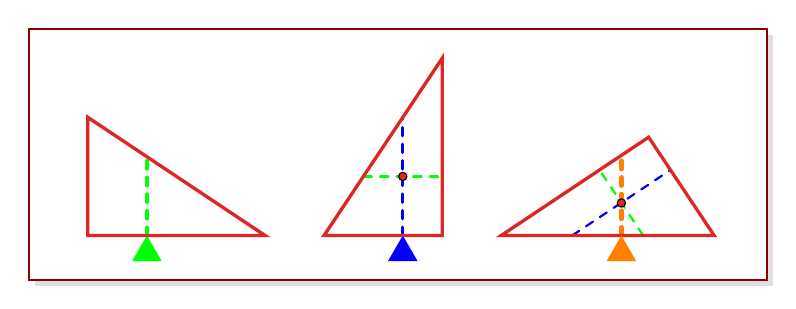
\begin{tikzpicture}[scale=0.75, line cap = round]

  \uncover<2->{
    \filldraw [white, draw=saitMaroon, thick, drop shadow={opacity=0.25}] (-1, -0.75) rectangle (11.5, 3.5);
    \fill[very thick, green] (1, 0) -- ++(-60:0.5) -- ++(180:0.5) -- cycle;
    \draw[very thick, dashed, green] (1,0) -- (1, 1.333);
    \draw[very thick, saitRed] (0, 0) -- (3, 0) -- (0,2) -- cycle;
  }
  \uncover<3->{
    \draw[thick, dashed, green] (4.667, 1) -- (6, 1);
    \fill[very thick, blue] (5.333, 0) -- ++(-60:0.5) -- ++(180:0.5) -- cycle;
    \draw[very thick, dashed, blue] (5.333, 0) -- ++(0, 2);
    \draw[very thick, saitRed] (4, 0) -- ++(2, 0) -- ++(0,3) -- cycle;
    \filldraw[fill=saitRed] (5.333,1) circle (2pt);% node[above right, inner sep=0.5mm]{$\bm C$};
  }
  \uncover<4>{
    \draw[thick, dashed, green] (9.404, 0) -- ++(123.69:1.333);
    \draw[thick, dashed, blue] (8.202, 0) -- ($ (7, 0) + (33.69:3) + (-56.31:0.667) $);
    \draw[ultra thick, dashed, orange] (9.0353, 0) -- (9.0353, 1.357);
    \draw[very thick, saitRed] (7, 0) -- ++(33.69:3) -- ++(-56.31:2) -- cycle;
    \fill[orange] (9.0353, 0) -- ++(-60:0.5) -- ++(180:0.5) -- cycle;
    % \node at (9.35,.5) (C2) ;
    \filldraw[fill=saitRed] (9.0353,.55) circle (2pt);% node[right, inner sep=1mm]{$\bm C$};
  }

\end{tikzpicture}

\end{frame}

%%%%%%%%%%%%%%%%%%%%%%%%%%%%%%%%%%%%%%%%%%%%%%%%%%%%%%%%%%%%%%%%%%%%%%%%%%%%%%%%
\begin{frame}{The Centre of Gravity}

	\cmini[0.8]{
		\begin{itemize}
			\item If the see-saw is in equilibrium (i.e., if it is static or `balanced'), then the line of action of centre of gravity of the board and the two children passes through the supporting log.
		\end{itemize}
	}
	\centering
	\cmini{
		\begin{statsbox}{}		
				\centering
				% !TEX root = ../../Beamer/04Centroids/04Centroids.tex
\def\scale{1}
\tikz[scale=\scale]{
  \coordinate (A) at (-2.675,0);
	\coordinate (B) at (-0.55,-0.25) node {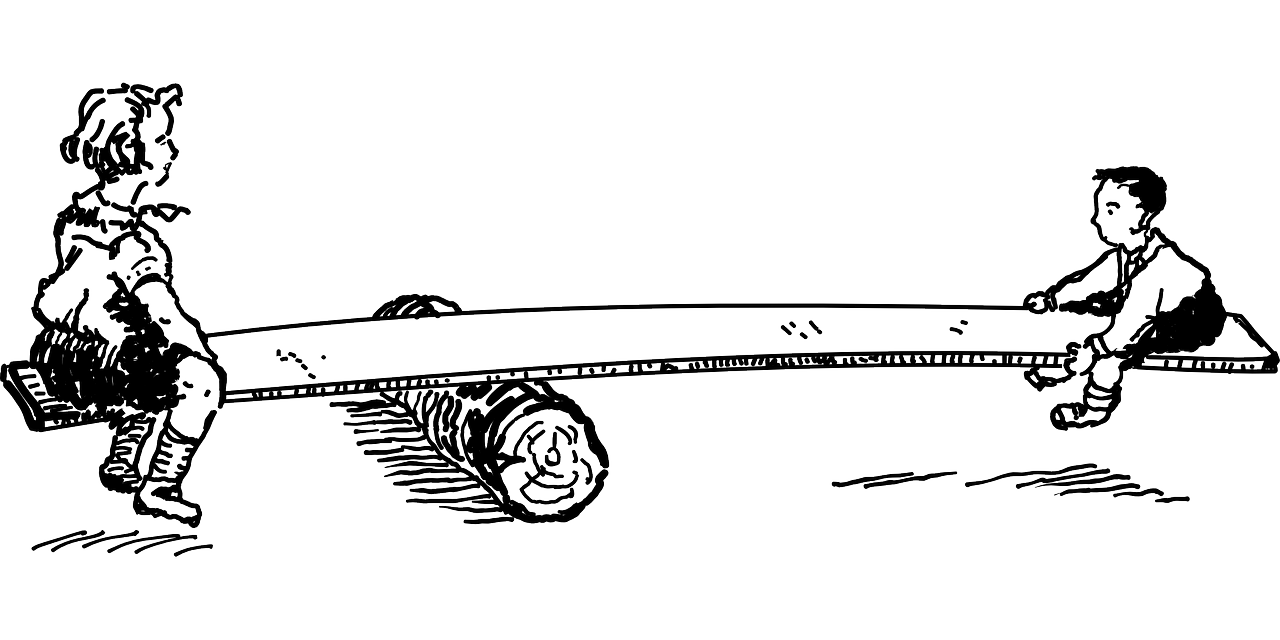
\includegraphics[scale=0.15]{../../images/teeter-totter.png}};
	\coordinate (C) at (2.8, 0);
  % \fill[mucus] ($ (A) - (1,1) $) rectangle ($ (C)+(1,1)  $);

  \draw [line width= 0.75mm,-latex, statsMaroon] (B) -- +(0,-1.2) node[below] {\Large $\bm G$};
}
		
		\end{statsbox}
	}
\end{frame}

%%%%%%%%%%%%%%%%%%%%%%%%%%%%%%%%%%%%%%%%%%%%%%%%%%%%%%%%%%%%%%%%%%%%%%%%%%%%%%%%

\begin{frame}{The Centroid}
	\centering
	\parm
	\def\scale{0.75}
	% !TEX root = ../all/statikz.tex

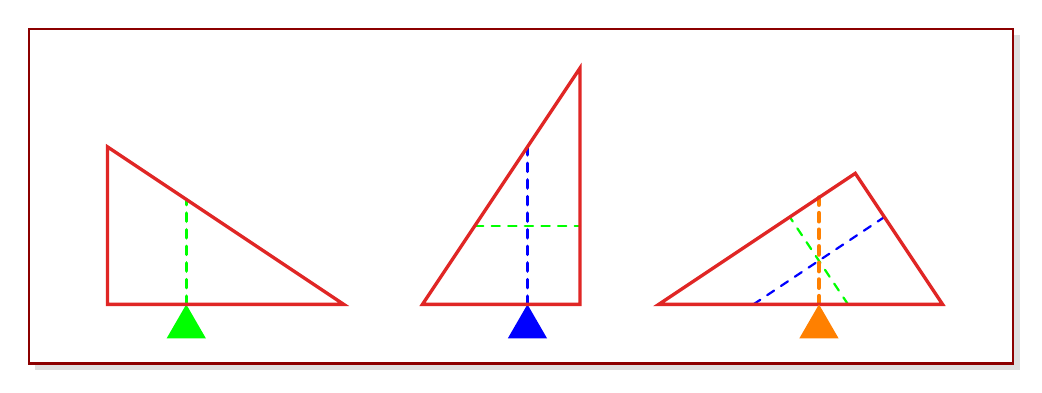
\begin{tikzpicture}[scale=\scale, line cap = round]

  \filldraw [white, draw=saitMaroon, thick, drop shadow={opacity=0.25}] (-1, -0.75) rectangle (11.5, 3.5);

  \fill[very thick, green] (1, 0) -- ++(-60:0.5) -- ++(180:0.5) -- cycle;
  \draw[very thick, dashed, green] (1,0) -- (1, 1.333);
  \draw[very thick, saitRed] (0, 0) -- (3, 0) -- (0,2) -- cycle;

  \draw[thick, dashed, green] (4.667, 1) -- (6, 1);
  \fill[very thick, blue] (5.333, 0) -- ++(-60:0.5) -- ++(180:0.5) -- cycle;
  \draw[very thick, dashed, blue] (5.333, 0) -- ++(0, 2);
  \draw[very thick, saitRed] (4, 0) -- ++(2, 0) -- ++(0,3) -- cycle;

  \draw[thick, dashed, green] (9.404, 0) -- ++(123.69:1.333);
  \draw[thick, dashed, blue] (8.202, 0) -- ($ (7, 0) + (33.69:3) + (-56.31:0.667) $);
  \draw[ultra thick, dashed, orange] (9.0353, 0) -- (9.0353, 1.357);
  \draw[very thick, saitRed] (7, 0) -- ++(33.69:3) -- ++(-56.31:2) -- cycle;
  \fill[orange] (9.0353, 0) -- ++(-60:0.5) -- ++(180:0.5) -- cycle;
\end{tikzpicture}


	\cmini[0.9]{
		\begin{itemize}
			\item  The resultant forces lines of action for the triangle shown assume a constant density of material.\parm
			\item If part of the triangle was constructed from steel and the rest from wood, the balance point might be very different.\parm
			\item But, if the body is of a uniform material, then the centre of gravity is at the geometric centre of the triangle shape. This geometric centre is called the {\bf centroid} of the area. \lb (You can think of it as the centre of gravity of the area.)\parm
			\item In civil engineering, we are mainly concerned with the centroid.
		\end{itemize}
	}
\end{frame}

%%%%%%%%%%%%%%%%%%%%%%%%%%%%%%%%%%%%%%%%%%%%%%%%%%%%%%%%%%%%%%%%%%%%%%%%%%%%%%%%
\begin{frame}{Centroids}

	\cmini[0.8]{
		The centroids of simple shapes are well-known. We shall just assume the results for these simple shapes: rectangles, triangles, circles, semi-circles and quarter circles
	}

	\begin{statsbox}{The Centroid of a Rectangle}%
		\footnotesize
		\mini[0.4]{
			% !TEX root = ../all/statikz.tex

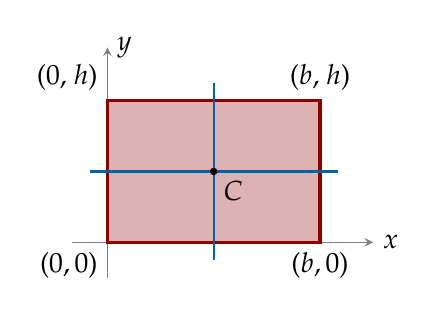
\begin{tikzpicture}[scale=0.9]
  \draw [gray, ->, >=stealth] (-0.5, 0) -- (3.75, 0) node[black, right] {$x$};
  \draw [gray, ->, >=stealth] (0, -0.5) -- (0, 2.75) node[black, right] {$y$};
  \filldraw[draw=saitMaroon, very thick, fill=saitMaroon!30!white] (0, 0) rectangle (3, 2);
  \node[below left] at (0, 0) {($0, 0$)};
  \node[below] at (3, 0) {($b, 0$)};
  \node[above] at (3, 2) {($b$, $h$)};
  \node[above left] at (0, 2) {($0$, $h$)};
  \uncover<2-4>{
    \draw[thick, saitDeepBlue] (1.5, 2.25) -- (1.5, -0.25);
  }
  \uncover<3-4>{
    \draw[thick, saitDeepBlue] (-0.25, 1) -- (3.25, 1);
  }
  \uncover<4->{
    \fill (1.5, 1) circle (1.5pt);
  }
  \uncover<5>{
    \node[below right] at (1.5, 1)  { $C$};
  }
\end{tikzpicture}

		}
		\hfill
		\mini[0.55]{
			\begin{itemize}
				\item<2-> The rectangle has a vertical axis of symmetry,  along the line $x=b/2$
				\item[]<3->	And a horizontal axis of symmetry along the line $y=h/2$.
				      \item<4-> If an area has an axis of symmetry, then the centroid will lie on that axis. In this case, the centroid must lie on both the vertical and the horizontal axes of symmetry.
				      \item<5> 	The centroid of the rectangle is at $$(\overline{x}, \overline{y}) = \left(\frac{b}{2}, \frac{h}{2}\right)$$ where $\overline{x}$ and $\overline{y}$ designate the $x$ and $y$ coordinates of the centroid.
			\end{itemize}
		}
	\end{statsbox}
\end{frame}

%%%%%%%%%%%%%%%%%%%%%%%%%%%%%%%%%%%%%%%%%%%%%%%%%%%%%%%%%%%%%%%%%%%%%%%%%%%%%%%

\begin{frame}{Centroids of Triangles}

	\cmini[0.9]{
		We focus on right triangles since they generally satisfy our needs.
	}

	\begin{statsbox}{The Centroid of a Right Triangle}
		\mini[0.45]{
			\footnotesize
			% !TEX root = ../all/statikz.tex

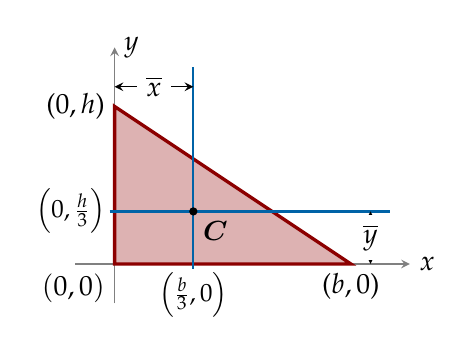
\begin{tikzpicture}

  \draw [gray, ->, >=stealth] (-0.5, 0) -- (3.75, 0) node[black, right] {$x$};
  \draw [gray, ->, >=stealth] (0, -0.5) -- (0, 2.75) node[black, right] {$y$};
  % \draw [help lines] (-0.5, -0.5) grid (3.5, 2.5);
  \filldraw[draw=saitMaroon, very thick, fill=saitMaroon!30!white] (0, 0) -- (3, 0) -- (0, 2) -- cycle;
  \node[below left] at (0, 0) {$(0, 0)$};
  \node[below] at (3, 0) {($b, 0$)};
  \node[left, scale=0.9] at (0, 0.667) {$\left(0, \frac{h}{3}\right)$};
  \node[below, scale=0.9] at (1, 0) {$\left(\frac{b}{3}, 0\right)$};
  \node[left] at (0, 2) {($0, h$)};
  \draw[thick, saitDeepBlue] (1, 2.5) -- (1, -0.0625);
  \draw[thick, saitDeepBlue] (-0.0625, 0.6667) -- (3.5, 0.6667);
  \fill (1, 0.667) circle (1.5pt) node[below right] {\normalsize  $\bm C$};  %{ $\left(\frac{b}{3}, \frac{h}{3}\right)$};
  \draw[<->, >=stealth] (0, 2.25) -- node[fill=white] {$\overline{x}$} (1, 2.25);
  \draw[<->, >=stealth] (3.25, 0) -- node[fill=white] {$\overline{y}$} (3.25, 0.667);

\end{tikzpicture}


		}
		\mini[0.5]{
			\begin{itemize}
				\item The centroid, $C$, of the triangle is located at $$\left(\overline{x}, \overline{y}\right) = \left(\frac{b}{3}, \frac{h}{3}\right) $$
			\end{itemize}
		}

	\end{statsbox}
\end{frame}

%%%%%%%%%%%%%%%%%%%%%%%%%%%%%%%%%%%%%%%%%%%%%%%%%%%%%%%%%%%%%%%%%%%%%%%%%%%%%%%

\begin{frame}{Centroids of Triangles (again)}

	\cmini[0.9]{
		The centroid of {\bfseries any} triangle is given by the average values of its vertices.
	}
	\begin{statsbox}{The Centroid of any Triangle}
		\mini[0.5]{
			\footnotesize
			% !TEX root = ../all/statikz.tex

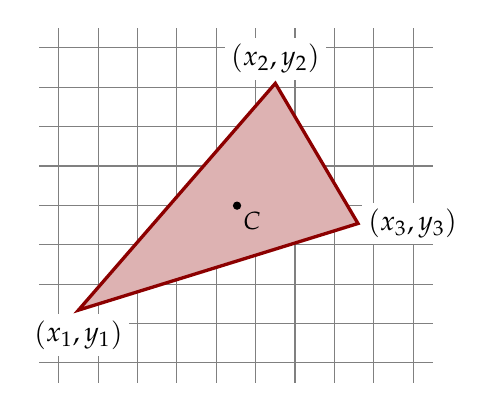
\begin{tikzpicture}[every node/.style={inner sep=.5ex}]
  \coordinate (A) at (-1.75, -1.33);
  \coordinate (B) at (0.75, 1.55);
  \coordinate (C) at (1.8, -0.23);


  \draw[gray, step=0.5cm]  (-2.25, -2.25) grid (2.75, 2.25);
  \filldraw[draw=saitMaroon, very thick, fill=saitMaroon!30!white, fill opacity = 0.75ex] (A) -- (B) -- (C) -- cycle;
  \node[below = 0.25ex, fill=white] at (A) {$\left(x_1, y_1\right)$};
  \node[above = 0.25ex, fill=white] at (B) {$\left(x_2, y_2\right)$};
  \node[right = 0.25ex, fill=white] at (C) {$\left(x_3, y_3\right)$};
  \normalsize
  \fill ($ 0.33*(A)+0.33*(B)+0.33*(C) $) circle (1.5pt)  node[below right, scale=0.9] {$C$};  %{ $\left(\frac{b}{3}, \frac{h}{3}\right)$};


\end{tikzpicture}

		}
		\mini[0.45]{
			\centering
			The centroid, $C$, of the triangle is located at \small $$\left(\frac{x_1+x_2+x_3}{3}, \frac{y_1+y_2+y_3}{3}\right) $$
		}
	\end{statsbox}
\end{frame}

%%%%%%%%%%%%%%%%%%%%%%%%%%%%%%%%%%%%%%%%%%%%%%%%%%%%%%%%%%%%%%%%%%%%%%%%%%%%%%%

\begin{frame}{Centroids of Parts of a Circle}

	% begin{textblock*}{width, e.g. 3cm}(x-coord eg 1cm, ycoord eg -0.5cm)
	\begin{textblock*}{1\textwidth}(1cm, 1.5cm)
		\centering
		The centroid of a circle is at the circle's centre \lb(the intersection of all axes of symmetry).\parm
		The semi-circle and the quarter-circle are less obvious.
	\end{textblock*}

	% begin{textblock*}{width, e.g. 3cm}(x-coord eg 1cm, ycoord eg -0.5cm)
	\begin{textblock*}{0.475\textwidth}(1cm, 3.5cm)
		\begin{statsbox}{Centroid of a Semi-Circle}{%
				\begin{center}
					% !TEX root = ../all/statikz.tex

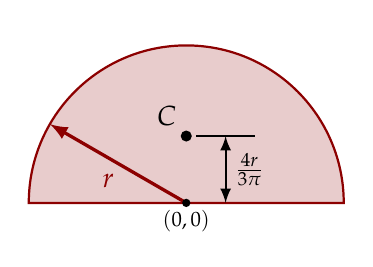
\begin{tikzpicture}
  \coordinate (center) at (0,0);
  \coordinate (C) at (0, 0.849);
  \filldraw[thick, fill=saitMaroon!20,draw=saitMaroon] (-2,0) -- (2,0) arc (0:180:2cm) -- (center);
  \draw[-latex, very thick, statsMaroon] (center) -- node[below,xshift=-0.125cm] {$r$} (150:2cm);
  \fill (center) circle (1.5pt);
  \fill (C) circle (2pt) node[above left] {$C$};
  \draw[latex-latex, thick] ($ (center) + (.5,0) $) -- node[right, scale=0.9] {$\frac{4r}{3\pi} $}($ (C) + (.5,0) $);
  \draw ($ (C) + (.125,0) $) -- ($ (C) + (.875,0) $);
  \node[below, scale=0.75] at (center) {$ (0,0) $};  
  \node[right, scale=0.75, white] at ($(center)+(0.75,2)$) {$ (0,r) $};
\end{tikzpicture}

					\footnotesize					
						$$\left(\overline{x}, \overline{y}\right) = \left(0, \frac{4r}{3\pi}\right) $$					
				\end{center}
			}
		\end{statsbox}
	\end{textblock*}

	\begin{textblock*}{0.475\textwidth}(6.75cm, 3.5cm)
		\begin{statsbox}{Centroid of a Quarter-Circle}{%
				\begin{center}					
					% !TEX root = ../all/statikz.tex

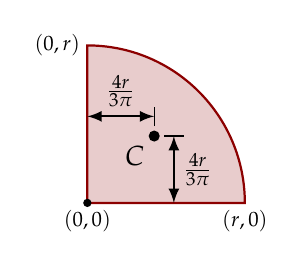
\begin{tikzpicture}
  \coordinate (center) at (0,0);
  \coordinate (C) at (0.849, 0.849);
  \filldraw[fill=saitMaroon!20,draw=saitMaroon, thick] (center) -- (2,0) arc (0:90:2cm) -- (center);
  \fill (center) circle (1.5pt);
  \fill (C) circle (2pt) node[below left] {$C$};
  \draw[latex-latex, thick] ($ (C) + (.25,0) $) -- node[right, scale=0.9] {$\frac{4r}{3\pi} $}($ (C) + (.25,-0.849) $);
  \draw[latex-latex, thick] ($ (C) + (0,.25) $) -- node[above, scale=0.9] {$\frac{4r}{3\pi} $}($ (C) + (-0.849,.25) $);
  \draw ($ (C) + (.125,0) $) -- ($ (C) + (.375,0) $);
  \draw ($ (C) + (0,.125) $) -- ($ (C) + (0,.375) $);
  % \draw[-latex, semithick] (center) -- node[sloped, below] {$r$} (0:2cm);
  \node[below, scale=0.75] at (center) {$ (0,0) $};
  \node[below, scale=0.75] at ($(center)+(2,0)$) {$ (r,0) $};
  \node[left, scale=0.75] at ($(center)+(0,2)$) {$ (0,r) $};
\end{tikzpicture}

					\footnotesize					
						$$\left(\overline{x}, \overline{y}\right) = \left(\frac{4r}{3\pi}, \frac{4r}{3\pi}\right) $$	
				\end{center}
			}
		\end{statsbox}
	\end{textblock*}
\end{frame}

%%%%%%%%%%%%%%%%%%%%%%%%%%%%%%%%%%%%%%%%%%%%%%%%%%%%%%%%%%%%%%%%%%%%%%%%%%%%%%%%

\begin{frame}{Simple Shape Exercises}
	\begin{myexer}{}{}
		\mini[0.45]{
			\footnotesize
			% !TEX root = ../all/statikz.tex

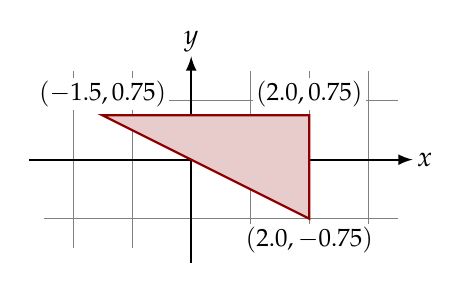
\begin{tikzpicture}[scale=0.75, every node/.style={inner sep=.25ex}]
	% \filldraw [white, draw=saitMaroon, thick, drop shadow={opacity=0.25}] (-0, 0) rectangle (3, 4);
	\coordinate (A) at (-1.5,0.75);
	\coordinate (B) at (2,-1);
	\coordinate (C) at (2,0.75);
	\draw[gray] (-2.5, -1.5) grid (3.5, 1.5);
	\draw [thick, black, -latex] (-2.75, 0) -- (3.75, 0) node[black, right] {$x$};
	\draw [thick, black, -latex] (0, -1.75) -- (0, 1.75) node[black, above] {$y$};
	\filldraw[thick, fill=saitMaroon!20,draw=saitMaroon] (A) -- (B) -- (C) -- cycle;
	\node[above = 0.35ex, fill=white] at (A) {\small $\left(-1.5, 0.75 \right)$};
	\node[below = 0.35ex, fill=white] at (B) {\small $\left(2.0, -0.75 \right)$};
	\node[above = 0.35ex, fill=white] at (C) {\small $\left(2.0, 0.75 \right)$};

\end{tikzpicture}

		}
		\hfill
		\mini[0.4]{
			Determine the location of the centroid of the triangle shown.
		}
	\end{myexer}
\end{frame}

%%%%%%%%%%%%%%%%%%%%%%%%%%%%%%%%%%%%%%%%%%%%%%%%%%%%%%%%%%%%%%%%%%%%%%%%%%%%%%%%

\begin{frame}{Simple Shape Exercises}
	\begin{myexer}{}{}
		\mini[0.45]{
			\footnotesize
			% !TEX root = ../all/statikz.tex

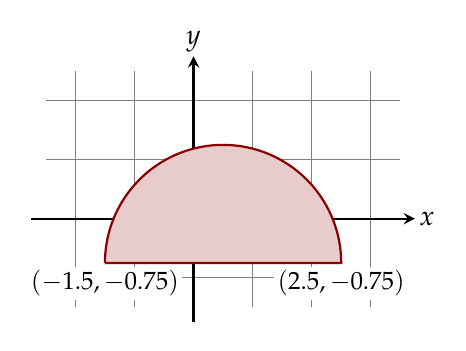
\begin{tikzpicture}[scale=0.75, every node/.style={inner sep=.25ex}]
  % \filldraw [white, draw=saitMaroon, thick, drop shadow={opacity=0.25}] (-0, 0) rectangle (3, 4);
  \coordinate (A) at (-1.5,-0.75);
  \coordinate (B) at (2.5,-0.75);
  \draw[gray] (-2.5, -1.5) grid (3.5, 2.5);
  \draw [thick, black, ->, >=stealth] (-2.75, 0) -- (3.75, 0) node[black, right] {$x$};
  \draw [thick, black, ->, >=stealth] (0, -1.75) -- (0, 2.75) node[black, above] {$y$};
  \filldraw[thick, fill=saitMaroon!20,draw=saitMaroon] (A) -- (B) arc (0:180:2cm);
  \node[below = 0.275ex, fill=white] at (A) {\small $\left(-1.5, -0.75\right)$};
  \node[below = 0.275ex, fill=white] at (B) {\small $\left(2.5, -0.75\right)$};

\end{tikzpicture}

		}
		\hfill
		\mini[0.4]{
			Determine the location of the centroid of the semi-circle shown.			
		}
	\end{myexer}
\end{frame}

%%%%%%%%%%%%%%%%%%%%%%%%%%%%%%%%%%%%%%%%%%%%%%%%%%%%%%%%%%%%%%%%%%%%%%%%%%%%%%%%

\begin{frame}{Simple Shape Exercises}
	\begin{myexer}{}{}
		\mini[0.45]{
			\footnotesize
			% !TEX root = ../all/statikz.tex

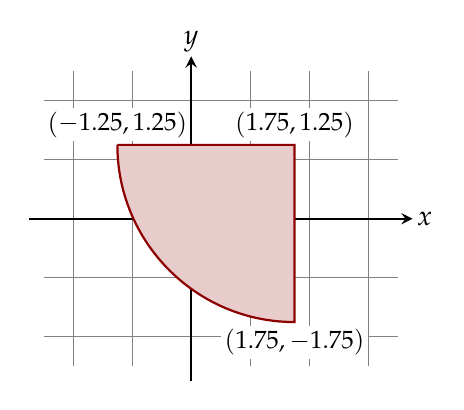
\begin{tikzpicture}[scale=0.75, every node/.style={inner sep=.25ex}]
	% \filldraw [white, draw=saitMaroon, thick, drop shadow={opacity=0.25}] (-0, 0) rectangle (3, 4);
	\coordinate (A) at (-1.25, 1.25);
	\coordinate (B) at (1.75,1.25);
	\coordinate (C) at (1.75,-1.75);
	\draw[gray] (-2.5, -2.5) grid (3.5, 2.5);
	\draw [thick, black, ->, >=stealth] (-2.75, 0) -- (3.75, 0) node[black, right] {$x$};
	\draw [thick, black, ->, >=stealth] (0, -2.75) -- (0, 2.75) node[black, above] {$y$};
	\filldraw[thick, fill=saitMaroon!20,draw=saitMaroon] (A) -- (B) -- (C) arc (270:180:3cm);
	\node[above = 0.275ex, fill=white] at (A) {\small $\left(-1.25, 1.25\right)$};
	\node[above = 0.275ex, fill=white] at (B) {\small $\left(1.75, 1.25\right)$};
	\node[below = 0.275ex, fill=white] at (C) {\small $\left(1.75, -1.75\right)$};

\end{tikzpicture}

		}
		\hfill
		\mini[0.4]{
			Determine the location of the centroid of the quarter-circle shown.
		}
	\end{myexer}
\end{frame}

%%%%%%%%%%%%%%%%%%%%%%%%%%%%%%%%%%%%%%%%%%%%%%%%%%%%%%%%%%%%%%%%%%%%%%%%%%%%%%%

\begin{frame}{Composite Shapes}
	Typically we are concerned with the properties of more complex shapes, composed of a number of simple shapes or standard structural cross-sections (such as wide-flange beams, channels, angles or plates).\parm

	Whether we are dealing with simple geometrical shapes or with standard sections, the centroid of the composite shape is given:
	\cmini[0.8]{
		\begin{statsbox}{Centroid of a Composite Shape}		
			{%
				\begin{align*}
					\overline{x} & = \frac{\Sigma Ax}{\Sigma A} = \frac{A_1 x_1 + A_2 x_2 + A_3 x_3 +\ldots}{A_1+A_2+A_3+\ldots} \\\\
					\overline{y} & = \frac{\Sigma Ay}{\Sigma A} = \frac{A_1 y_1 + A_2 y_2 + A_3 y_3 +\ldots}{A_1+A_2+A_3+\ldots}
				\end{align*}
				\cmini[0.8]{
					where the $A_i$ are the areas of the simple shapes making up the composite shape and the $x_i$ and $y_i$ are the $\overline{x}$ and the ${\overline{y}}$ of the simple shapes.
				}
			}
		\end{statsbox}
	}
\end{frame}
%%%%%%%%%%%%%%%%%%%%%%%%%%%%%%%%%%%%%%%%%%%%%%%%%%%%%%%%%%%%%%%%%%%%%%%%%%%%%%%%
\begin{frame}{Composite Shapes}
	\begin{myexam}[height=7cm]{}{}
		\vspace{0.5cm}
		\mini[0.55]{
			% !TEX root = ../all/statikz.tex

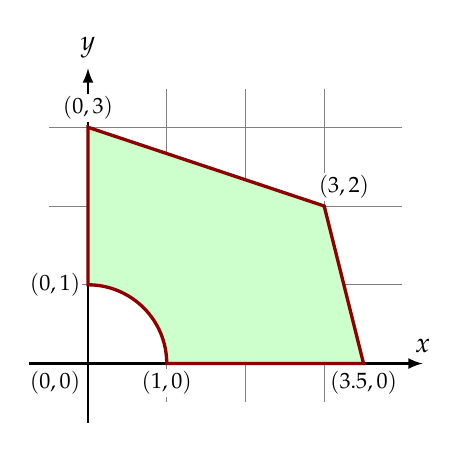
\begin{tikzpicture}[scale=\scale]
	\draw[gray, step=1cm] (-0.49,-0.49) grid (3.99,3.49);
	\draw[-latex, thick, black] (-0.75, 0) -- (4.25, 0) node[above] {$x$};
	\draw[-latex, thick, black] (0, -0.75) -- (0,3.75) node[above] {$y$};
	\filldraw[draw=saitMaroon, fill=green!20, very thick] (0,1) arc(90:0:1)-- (3.5, 0) -- (3,2) -- (0,3) -- cycle;

	\footnotesize
	\node[below left, fill=white, inner sep=0.1em, outer sep=0.25em] at (0,0) { $(0, 0)$};
	\node[below, fill=white, inner sep=0.1em, outer sep=0.25em] at (1,0) { $(1, 0)$};
	\node[below, fill=white, inner sep=0.1em, outer sep=0.25em] at (3.5,0) { $(3.5, 0)$};
	\node[above, fill=white, inner sep=0.1em, outer sep=0.25em] at (3.25,2) { $(3, 2)$};
	\node[above, fill=white, inner sep=0.1em, outer sep=0.25em] at (0,3) { $(0, 3)$};
	\node[left, fill=white, inner sep=0.1em, outer sep=0.25em] at (0,1) { $(0, 1)$};


\end{tikzpicture}

		}
		\hfill
		\mini[0.4]{
			Find the location of the centroid, $C$, relative to the coordinate origin.
		}
		\addtocounter{\tcbcounter}{-1}
	\end{myexam}
\end{frame}

%%%%%%%%%%%%%%%%%%%%%%%%%%%%%%%%%%%%%%%%%%%%%%%%%%%%%%%%%%%%%%%%%%%%%%%%%%%%%%%%
\begin{frame}{Composite Shapes}
	\begin{myexam}[height=7cm]{Solution}{}
			\vspace{0.5cm}
		\mini[0.5]{
			% \def\scale{0.8}
			% !TEX root = ../all/statikz.tex

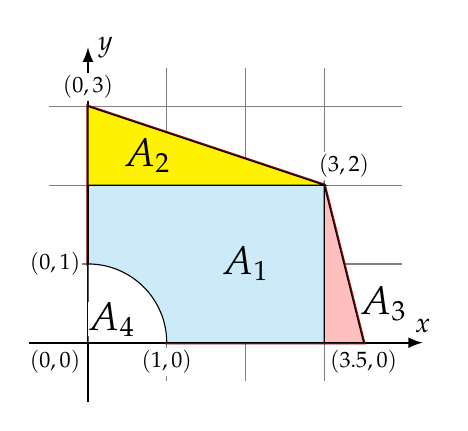
\begin{tikzpicture}[scale=\scale]
	\draw[gray] (-0.49,-0.49) grid (3.99,3.49);
	\draw[-latex, thick, black] (-0.75, 0) -- (4.25, 0) node[above] {$x$};
	\draw[-latex, thick, black] (0, -0.75) -- (0,3.75) node[right] {$y$};
	\filldraw[draw=saitMaroon, fill=green!20, very thick] (0,1) arc(90:0:1)-- (3.5, 0) -- (3,2) -- (0,3) -- cycle;

	\footnotesize
	\node[below left, fill=white, inner sep=0.1em, outer sep=0.25em] at (0,0) { $(0, 0)$};
	\node[below, fill=white, inner sep=0.1em, outer sep=0.25em] at (1,0) { $(1, 0)$};
	\node[below, fill=white, inner sep=0.1em, outer sep=0.25em] at (3.5,0) { $(3.5, 0)$};
	\node[above, fill=white, inner sep=0.1em, outer sep=0.25em] at (3.25,2) { $(3, 2)$};
	\node[above, fill=white, inner sep=0.1em, outer sep=0.25em] at (0,3) { $(0, 3)$};
	\node[left, fill=white, inner sep=0.1em, outer sep=0.25em] at (0,1) { $(0, 1)$};

	\uncover<2->{
		\filldraw[fill=saitBlue!20] (0,0) rectangle (3,2);
		\node at (2,1) {\Large $A_1$};
		\filldraw[fill=yellow] (0,2) -- (3,2) -- (0,3) -- cycle;
		\node at (0.75,2.375) {\Large $A_2$};
		\filldraw[fill=pink] (3,0) -- (3,2) -- (3.5,0) -- cycle;
		\node[fill=white, inner sep=0] at (3.75,0.5) {\Large $A_3$};
	}
  \uncover<3->{
  \filldraw[fill=white] (0,0) -- (1,0)arc(0:90:1) -- cycle;
  \node[fill=white, inner sep=0] at (0.3,0.3) {\Large $A_4$};
  }


\end{tikzpicture}

		}
		\hfill
		\mini[0.45]{
			\begin{enumerate}
				\item Divide the composite shape into simple shapes:\pause
				      \begin{itemize}
				      	\item Notice that the `missing' quarter-circle is covered up by rectangle $A_1$.\pause
				      	\item Draw in the quater-circle; we shall treat this area as negative\pause
				      \end{itemize}
				\item Apply the formul\ae{} for $\overline{x}$ and $\overline{y}$.
				\item For complicated shapes, you may want to arrange your data in a table.
			\end{enumerate}
		}

		\addtocounter{\tcbcounter}{-1}
	\end{myexam}
\end{frame}

%%%%%%%%%%%%%%%%%%%%%%%%%%%%%%%%%%%%%%%%%%%%%%%%%%%%%%%%%%%%%%%%%%%%%%%%%%%%%%%%
\begin{frame}{Composite Shapes}
	\begin{myexam}[height=7cm]{Solution}{}
			\vspace{0.35cm}
		\mini[0.325]{
			\def\scale{0.6}
			% !TEX root = ../all/statikz.tex

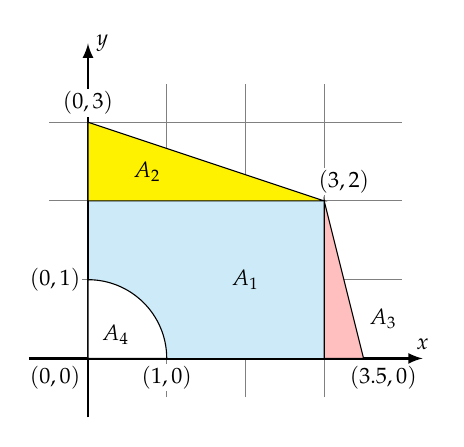
\begin{tikzpicture}[scale=\scale]
  \footnotesize
	\draw[gray] (-0.49,-0.49) grid (3.99,3.49);
	\draw[-latex, thick, black] (-0.75, 0) -- (4.25, 0) node[above] {$x$};
	\draw[-latex, thick, black] (0, -0.75) -- (0,4) node[right] {$y$};
	

	\node[below left, fill=white, inner sep=0.1em, outer sep=0.25em] at (0,0) { $(0, 0)$};
	\node[below, fill=white, inner sep=0.1em, outer sep=0.25em] at (1,0) { $(1, 0)$};
	\node[below, fill=white, inner sep=0.1em, outer sep=0.25em] at (3.75,0) { $(3.5, 0)$};
	\node[above, fill=white, inner sep=0.1em, outer sep=0.25em] at (3.25,2) { $(3, 2)$};
	\node[above, fill=white, inner sep=0.1em, outer sep=0.25em] at (0,3) { $(0, 3)$};
	\node[left, fill=white, inner sep=0.1em, outer sep=0.25em] at (0,1) { $(0, 1)$};

		\filldraw[fill=saitBlue!20] (0,0) rectangle (3,2);
		\node at (2,1) { $A_1$};
		\filldraw[fill=yellow] (0,2) -- (3,2) -- (0,3) -- cycle;
		\node at (0.75,2.375) { $A_2$};
		\filldraw[fill=pink] (3,0) -- (3,2) -- (3.5,0) -- cycle;
		\node[fill=white, inner sep=0] at (3.75,0.5) { $A_3$};

  \filldraw[fill=white] (0,0) -- (1,0)arc(0:90:1) -- cycle;
  \node[fill=white, inner sep=0] at (0.35,0.3) { $A_4$};
  % }


\end{tikzpicture}

		}
		\hfill
		\mini[0.675]{
			\footnotesize
			\begin{align*}
				\overline{x} & = \frac{A_1x_1+A_2x_2+A_3x_3+A_4x_4}{A_1+A_2+A_3+A_4}                                                        \\
				             & = \frac{6(1.5)+1.5(1)+0.5(3.1667)-\frac{\pi}{4}\left(\frac{4\times 1}{3\pi}\right)}{6+1.5+0.5-\frac{\pi}{4}} \\
				             & = \frac{11.750}{7.2146} = 1.6286                                                                             \\\\
				\overline{y} & = \frac{A_1y_1+A_2y_2+A_3y_3+A_4y_4}{A_1+A_2+A_3+A_4}                                                        \\
				             & =    \frac{6(1)+1.5(2.3333)+0.5(0.66667)-\frac{\pi}{4}\left(\frac{4\times 1}{3\pi}\right)}{7.2146}           \\
				             & =   \frac{9.5000}{7.2146} = 1.3168
			\end{align*}

		}
		\parb
		\centering
		\normalsize
		The centroid is at the location $\left(\overline{x},\overline{y}\right)=(1.63,1.32)$.
		\addtocounter{\tcbcounter}{-1}
	\end{myexam}
\end{frame}

%%%%%%%%%%%%%%%%%%%%%%%%%%%%%%%%%%%%%%%%%%%%%%%%%%%%%%%%%%%%%%%%%%%%%%%%%%%%%%%%
\begin{frame}{Composite Shapes}
	\begin{myexam}[height=7cm]{Solution Using Table}{}
		\small
			\vspace{0.8cm}
		\centering
		\begin{tabular}{cccccc}
			Shape            & Area                          & $x_i$               & $y_i$               & $A_ix_i$                        & $A_iy_i$                        \\
			\addlinespace
			\midrule
			$A_1$            & $6.0000$                      & $1.5000$            & $1.0000$            & \textcolor{saitRed}{$9.0000$}   & \textcolor{saitRed}{$6.0000$}   \\
			\midrule
			$A_2$            & $1.5000$                      & $1.0000$            & $2.3333$            & \textcolor{saitRed}{$1.5000$}   & \textcolor{saitRed}{$3.5000$}   \\
			\midrule
			$A_3$            & $0.50000$                     & $3.1667$            & $0.66667$           & \textcolor{saitRed}{$1.5834$}   & \textcolor{saitRed}{0.33333}    \\
			\midrule
			$A_4$            & $\bm -\frac{\pi}{4}$          & $\frac{4(1)}{3\pi}$ & $\frac{4(1)}{3\pi}$ & \textcolor{saitRed}{$-0.33333$} & \textcolor{saitRed}{$-0.33333$} \\
			\bottomrule\addlinespace
			{\Large$\Sigma$} & \textcolor{saitRed}{$7.2146$} &                     &                     & \textcolor{saitRed}{$11.750$}   & \textcolor{saitRed}{$9.5000$}
		\end{tabular}

		\parb
		\centering
		\normalsize
		$$\left(\overline{x},\overline{y}\right)=\left(\frac{\Sigma A_ix_i}{A},\frac{\Sigma A_iy_i}{A}\right)=\left(\frac{11.750}{7.2146}, \frac{9.5000}{7.2146}\right)=(1.63,1.32)$$
		\addtocounter{\tcbcounter}{-1}
	\end{myexam}
\end{frame}

%%%%%%%%%%%%%%%%%%%%%%%%%%%%%%%%%%%%%%%%%%%%%%%%%%%%%%%%%%%%%%%%%%%%%%%%%%%%%%%
\begin{frame}{Composite Shapes}
	\begin{myexam}[height=7cm]{The Answer}{}
		\centering
		\vspace{0.5cm}
		\def\scale{1}
		% !TEX root = ../all/statikz.tex

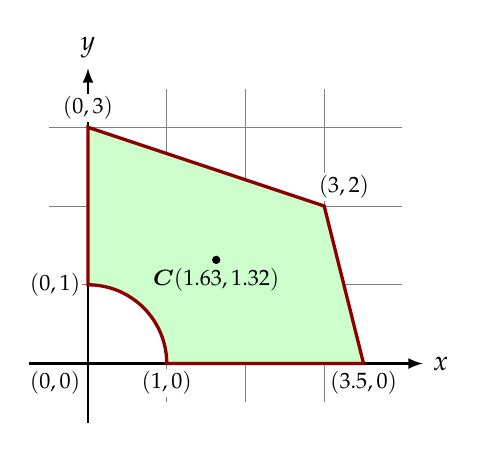
\begin{tikzpicture}[scale=\scale]
  \draw[gray, step=1cm] (-0.49,-0.49) grid (3.99,3.49);
  \draw[-latex, thick, black] (-0.75, 0) -- (4.25, 0) node[right] {$x$};
  \draw[-latex, thick, black] (0, -0.75) -- (0,3.75) node[above] {$y$};
  \filldraw[draw=saitMaroon, fill=green!20, very thick] (0,1) arc(90:0:1)-- (3.5, 0) -- (3,2) -- (0,3) -- cycle;

  \footnotesize
  \node[below left, fill=white, inner sep=0.1em, outer sep=0.25em] at (0,0) { $(0, 0)$};
  \node[below, fill=white, inner sep=0.1em, outer sep=0.25em] at (1,0) { $(1, 0)$};
  \node[below, fill=white, inner sep=0.1em, outer sep=0.25em] at (3.5,0) { $(3.5, 0)$};
  \node[above, fill=white, inner sep=0.1em, outer sep=0.25em] at (3.25,2) { $(3, 2)$};
  \node[above, fill=white, inner sep=0.1em, outer sep=0.25em] at (0,3) { $(0, 3)$};
  \node[left, fill=white, inner sep=0.1em, outer sep=0.25em] at (0,1) { $(0, 1)$};



   \coordinate (C) at (1.6287,1.3168);
   \fill (C) circle (1.5pt) node[below] {$\bm C(1.63, 1.32)$};

\end{tikzpicture}

	\end{myexam}
\end{frame}

%%%%%%%%%%%%%%%%%%%%%%%%%%%%%%%%%%%%%%%%%%%%%%%%%%%%%%%%%%%%%%%%%%%%%%%%%%%%%%%%
\begin{frame}{Composite Shapes}
	\begin{myexer}{}{}
		\small
		\mini[0.65]{
			% !TEX root = ../all/statikz.tex



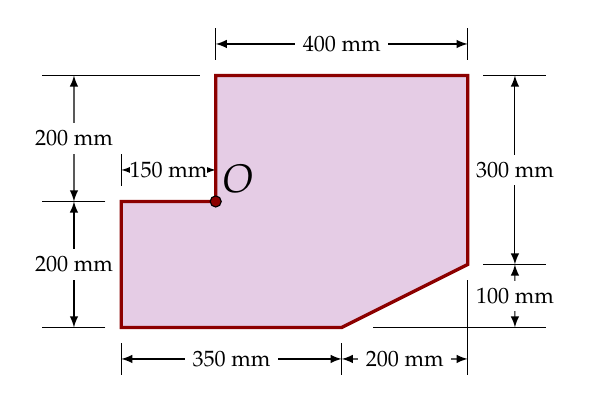
\begin{tikzpicture}[scale=0.8]

  \coordinate (O) at (0,0);
  \coordinate (B) at (0,2);
  \coordinate (C) at (4,2);
  \coordinate (D) at (4,-1);
  \coordinate (E) at (2,-2);
  \coordinate (F) at (-1.5,-2);
  \coordinate (G) at (-1.5,0);

  \draw ($ (B)+(0,0.25) $) -- +(0,.5);
  \draw ($ (C)+(0,0.25) $) -- +(0,.5);
  \draw ($ (G)+(0,0.25) $) -- +(0,0.5);

  \draw ($ (C)+(0.25, 0) $) -- +(1,0);
  \draw ($ (D)+(0.25, 0) $) -- +(1,0);
  \draw ($ (E)+(0.5, 0) $) -- +(2.75,0);

  \draw ($ (D)+(0, -0.25) $) -- +(0,-1.5);
  \draw ($ (E)+(0, -0.25) $) -- +(0,-.5);
  \draw ($ (F)+(0, -0.25) $) -- +(0,-.5);

  \draw ($ (F)+(-0.25, 0) $) -- +(-1,0);
  \draw ($ (G)+(-0.25, 0) $) -- +(-1,0);
  \draw ($ (B)+(-0.25, 0) $) -- +(-2.5,0);

  \footnotesize

  \draw[latex-latex] ($ (B)+(0,0.5) $) -- node[fill=white]{400 mm} ($ (C)+(0,0.5) $);
  \draw[latex-latex] ($ (G)+(0,0.5) $) -- node[fill=white, inner sep=0]{150 mm} ($ (O)+(0,0.5) $);
  \draw[latex-latex] ($ (D)-(0,1.5) $) -- node[fill=white]{200 mm} ($ (E)-(0,0.5) $);
  \draw[latex-latex] ($ (E)-(0,0.5) $) -- node[fill=white]{350 mm} ($ (F)-(0,0.5) $);
  \draw[latex-latex] ($ (C)+(0.75,0) $) -- node[fill=white]{300 mm} ($ (D)+(0.75,0) $);
  \draw[latex-latex] ($ (D)+(0.75,0) $) -- node[fill=white]{100 mm} ($ (E)+(2.75,0) $);
  \draw[latex-latex] ($ (F)-(0.75,0) $) -- node[fill=white]{200 mm} ($ (G)-(0.75,0) $);
  \draw[latex-latex] ($ (G)-(0.75,0) $) -- node[fill=white]{200 mm} ($ (B)-(2.25,0) $);


  % \draw[gray] (-1.9,-2.49) grid (4.49,2.49);
  % \draw[-latex, thick, black] (-2.25, 0) -- (4.75, 0) node[right] {$x$};
  % \draw[-latex, thick, black] (0, -2.75) -- (0,2.75) node[above] {$y$};
  \filldraw[draw=saitMaroon, fill=violet!20!white, very thick] (O) -- (B) -- (C) -- (D) -- (E) -- (F) -- (G) -- cycle;
  \filldraw[fill=saitMaroon, draw=black] (O) circle (2.5pt);
  \footnotesize

  \node[above right, inner sep=0.1em, outer sep=0.25em] at (0,0) {\Large $O$};
  % \node[above left, fill=white, inner sep=0.1em, outer sep=0.25em] at (-1.3,0) { $(-1.3, 0)$};
  % \node[below, fill=white, inner sep=0.1em, outer sep=0.25em] at (-1.3,-1.7) { $(-1.3, -1.7$};
  % \node[below, fill=white, inner sep=0.1em, outer sep=0.25em] at (2,-1.7) { $(2, -1.7)$};
  % \node[above, fill=white, inner sep=0.1em, outer sep=0.25em] at (4.1,1.9) { $(4.1, 1.9)$};
  % \node[above, fill=white, inner sep=0.1em, outer sep=0.25em] at (0,1.9) { $(0, 1.9)$};
  % \node[below, fill=white, inner sep=0.1em, outer sep=0.25em] at (4.5,-0.675) { $(4.1, -1.5)$};

\end{tikzpicture}

		}
		\hfill
		\mini[0.25]{
			Find the location of the centroid, $C$, relative to the point~$O$.
		}

	\end{myexer}
\end{frame}

%%%%%%%%%%%%%%%%%%%%%%%%%%%%%%%%%%%%%%%%%%%%%%%%%%%%%%%%%%%%%%%%%%%%%%%%%%%%%%%%

\begin{frame}{Composite Shapes}
	\begin{myexer}{}{}
		\mini[0.65]{
			% !TEX root = ../all/statikz.tex

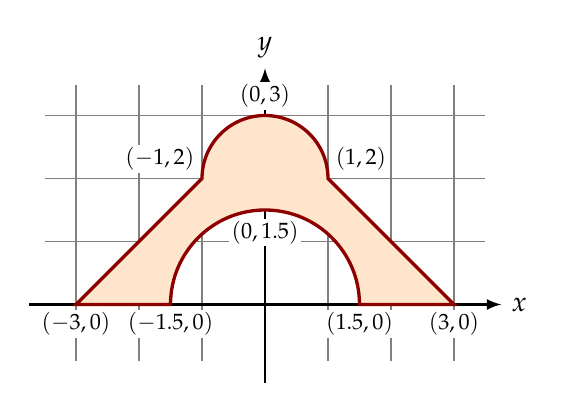
\begin{tikzpicture}[scale=0.8]
  \draw[gray] (-3.5,-.9) grid (3.5,3.49);
  \draw[-latex, thick, black] (-3.75, 0) -- (3.75, 0) node[right] {$x$};
  \draw[-latex, thick, black] (0, -1.25) -- (0,3.75) node[above] {$y$};
  \filldraw[draw=saitMaroon, fill=orange!20!white, very thick] (-1.5,0) -- (-3, 0) -- (-1, 2) arc (180:0:1) -- (3,0)  -- (1.5,0) arc (0:180:1.5) -- cycle;
  \footnotesize

  \node[below, fill=white, inner sep=0.1em, outer sep=0.25em] at (-1.5,0) { $(-1.5, 0)$};
  \node[below, fill=white, inner sep=0.1em, outer sep=0.25em] at (-3,0) { $(-3, 0)$};
  \node[above left, fill=white, inner sep=0.1em, outer sep=0.25em] at (-1,2) { $(-1, 2)$};
  \node[above right, fill=white, inner sep=0.1em, outer sep=0.25em] at (1,2) { $(1, 2)$};
  \node[below, fill=white, inner sep=0.1em, outer sep=0.25em] at (3,0) { $(3, 0)$};
  \node[below, fill=white, inner sep=0.1em, outer sep=0.25em] at (1.5,0) { $(1.5, 0)$};
  \node[below, fill=white, inner sep=0.1em, outer sep=0.25em] at (0,1.45) { $(0, 1.5)$};
  \node[above, fill=white, inner sep=0.1em, outer sep=0.25em] at (0,3) { $(0,3)$};

\end{tikzpicture}

		}
		\hfill
		\mini[0.3]{
			Find the location of the centroid, $C$, relative to the coordinate origin.			
		}
	\end{myexer}
\end{frame}

%%%%%%%%%%%%%%%%%%%%%%%%%%%%%%%%%%%%%%%%%%%%%%%%%%%%%%%%%%%%%%%%%%%%%%%%%%%%%

\begin{frame}{Structural Steel}
	\centering
	\cfig[0.25]{../../images/2011-07-10-211.jpg}

	\cmini[0.8]{
		\centering
		This modern Calgary high-rise contains a lot of steel...
	}

\end{frame}

%%%%%%%%%%%%%%%%%%%%%%%%%%%%%%%%%%%%%%%%%%%%%%%%%%%%%%%%%%%%%%%%%%%%%%%%%%%%%

\begin{frame}{Structural Steel}
	\centering
	\cfig[0.20]{../../images/2009-04-18-052.jpg}

	\cmini[0.8]{
		\centering
		Just some of the steel that went into the highrise...
	}
\end{frame}

%%%%%%%%%%%%%%%%%%%%%%%%%%%%%%%%%%%%%%%%%%%%%%%%%%%%%%%%%%%%%%%%%%%%%%%%%%%%%

\begin{frame}{Structural Steel}
	\centering
	\cfig[0.35]{../../images/steelSections}
	\begin{itemize}
		\item There are many structural steel sections used in construction.
		\item Details of their physical dimensions and structural properties are widely available in tables. 	     
		\item Often, various sections are welded together to suit a particular need.
	\end{itemize}

\end{frame}

%%%%%%%%%%%%%%%%%%%%%%%%%%%%%%%%%%%%%%%%%%%%%%%%%%%%%%%%%%%%%%%%%%%%%%%%%%%%%

\begin{frame}{Wide-flanged I-beams}

	\mini[0.3]{
		\centering
		% !TEX root = ../all/statikz.tex



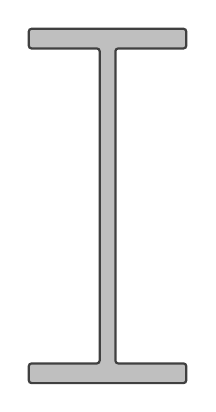
\begin{tikzpicture}[scale=\scale]
  % \draw[gray] (-3.5,-.9) grid (3.5,3.49);
  % \draw[->, >=stealth, thick, black] (-3.75, 0) -- (3.75, 0) node[right] {$x$};
  % \draw[->, >=stealth, thick, black] (0, -1.25) -- (0,3.75) node[above] {$y$};
  \filldraw[rounded corners=1pt, draw=gray!50!black, fill=gray!50!white, thick] (0,0) -- (2, 0) -- (2,.25) -- (1.1,0.25)  -- (1.1,4.25) -- (2,4.25) -- (2,4.5) -- (0,4.5) -- (0,4.25) -- (0.9,4.25) -- (0.9,0.25) -- (0,0.25) -- cycle;


\end{tikzpicture}

	}
	\hfill
	\mini[0.65]{
		\begin{itemize}
			\item  A common beam used in construction has this characteristic I-shaped cross-section.
			\item This is called a wide-flanged I-beam due to the large horizontal flanges top and bottom.
			\item It has three parts: top and bottom horizontal {\bfseries flanges} and a vertical {\bfseries web}.
			% \item Properties of these beams can be read from table A.3 (see page 459 in your textbook).
			\item These beams are designated in the form\\ \textcolor{saitRed}{W depth x mass per unit length}.\par
			\item A W460x82 beam has a wide flange (hence the W), a nominal depth of 460mm and a mass of 82 kg per metre.

		\end{itemize}
	}
\end{frame}

%%%%%%%%%%%%%%%%%%%%%%%%%%%%%%%%%%%%%%%%%%%%%%%%%%%%%%%%%%%%%%%%%%%%%%%%%%%%%

\begin{frame}{Wide-flanged I-beams}

	\mini[0.3]{
		\centering
		% !TEX root = ../all/statikz.tex



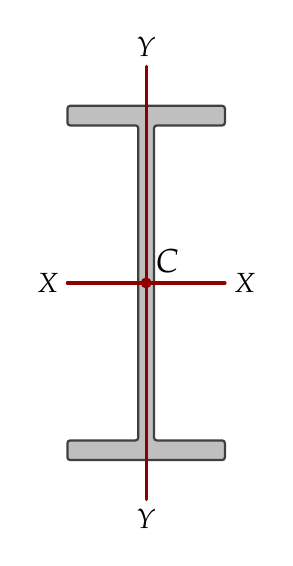
\begin{tikzpicture}[scale=\scale, line cap = round]
	% \draw[gray] (-3.5,-.9) grid (3.5,3.49);
	% \draw[->, >=stealth, thick, black] (-3.75, 0) -- (3.75, 0) node[right] {$x$};
	% \draw[->, >=stealth, thick, black] (0, -1.25) -- (0,3.75) node[above] {$y$};
	\filldraw[rounded corners=1pt, draw=gray!50!black, fill=gray!50!white, thick] (0,0) -- (2, 0) -- (2,.25) -- (1.1,0.25)  -- (1.1,4.25) -- (2,4.25) -- (2,4.5) -- (0,4.5) -- (0,4.25) -- (0.9,4.25) -- (0.9,0.25) -- (0,0.25) -- cycle;

	\draw[very thick, statsMaroon] (1,-0.5) -- (1,5);
	\draw[very thick, statsMaroon] (0,2.25) -- (2,2.25);
	\fill[statsMaroon] (1,2.25) circle (2pt) node[above right, black] {\large $C$};
	\node at  (-0.25,2.25) {$X$};
	\node at  (2.25,2.25) {$X$};
	\node at  (1,-.75) {$Y$};
	\node at  (1,5.25) {$Y$};

\end{tikzpicture}

	}
	\hfill
	\mini[0.65]{
		\begin{itemize}
			\item  The beam has a vertical axis of symmetry so the centroid must be on that line.\parb
			\item The beam also has a horizontal axis of symmetry so the centroid must be on that line, too.\parb
			\item The centroid of the cross-sectional area of the beam is easily found at the intersection of the two axes of symmetry.


		\end{itemize}
	}
\end{frame}

%%%%%%%%%%%%%%%%%%%%%%%%%%%%%%%%%%%%%%%%%%%%%%%%%%%%%%%%%%%%%%%%%%%%%%%%%%%%%

\begin{frame}{Structural Steel}

	\begin{textblock*}{0.5\textwidth}(0.5cm, 1cm)
		\centering
		\cfig[0.14]{../../images/080914_22.jpg}
		\mini[0.8]{
			\centering
			One of these beams may support your floor system at home...
		}


	\end{textblock*}

	\begin{textblock*}{0.5\textwidth}(6.2cm, 2cm)
		\centering
		\cfig[0.14]{../../images/2011-05-18-062.jpg}
		\hfill
		\mini[0.6]{
			\centering
		...or the ceiling above my office...}
	\end{textblock*}
\end{frame}

%%%%%%%%%%%%%%%%%%%%%%%%%%%%%%%%%%%%%%%%%%%%%%%%%%%%%%%%%%%%%%%%%%%%%%%%%%%%%

\begin{frame}{Built-up Structural Steel Sections}
	\begin{myexam}{}{}
		\mini[0.5]{
			\centering
			\def\scale{0.85}
			% !TEX root = ../all/statikz.tex

\tikz[scale=\scale]{

  \def\phil{gray!50!white}
  \def\stroke{black}

  \begin{scope}[scale=\scale]

    \filldraw[rounded corners=1pt, draw=\stroke, fill=\phil, thick] (-2.5, 1.5) rectangle (2.5,2.125);

    \coordinate (A) at (-1.5,0);
    \coordinate (B) at (1.5,0);

    \WBeam{A}{\phil}{\stroke}{0.5}{1}
    \WBeam{B}{\phil}{\stroke}{0.5}{1}

  \end{scope}
}


		}
		\hfill
		\mini[0.45]{
			Two W250X115 steel beams have a steel plate welded on top of them, as shown. The dimensions of the plate are 650 mm x 60 mm.\parb
			How far below the top of the built-up section is the centroidal $x$-axis?
			\parb
			\footnotesize
			\centering
			\textcolor{statsMaroon}{
			From the beam tables for W250X115:\lb
			Area $= 14600\,\mathsf{mm^2}$\lb
			Depth $=269\,\mathsf{mm}$}
			
		}
		\addtocounter{\tcbcounter}{-1}
	\end{myexam}

\end{frame}

\begin{frame}{Built-up Structural Steel Sections}
	\begin{myexam}{Solution}{}
		\mini[0.4]{
		\def\scale{0.55}
			% !TEX root = ../all/statikz.tex

\tikz[scale=\scale]{


  \def\phil{gray!50!white}
  \def\stroke{black}

  % \begin{scope}[scale=\scale]
    \draw[gray, -latex] (-3.5,2.125) -- (3.5,2.125) node[above] {$x$};
    \draw[gray, -latex] (0,-2) -- (0,3) node[right] {$y$};
    \node at (-2,-0.5) {\footnotesize$A_1$};
    \node at (2,-0.5) {\footnotesize$A_2$};
    \node at (2,2.375) {\footnotesize$A_3$};
    \filldraw[rounded corners=1pt, draw=\stroke, fill=\phil, thick] (-2.5, 1.5) rectangle (2.5,2.125);

    \coordinate (A) at (-1.5,0);
    \coordinate (B) at (1.5,0);

    \WBeam{A}{\phil}{\stroke}{0.5}{1}
    \WBeam{B}{\phil}{\stroke}{0.5}{1}

  % \end{scope}
}


		}
		\hfill
		\mini[0.55]{
			\centering\small
			\begin{tabular}{cccc}
				Shape    & $A_i$                            & $y_i$                          & $A_iy_i$                         \\
				         & \footnotesize$\mathsf{\;(mm^2)}$ & \footnotesize$\mathsf{\;(mm)}$ & \footnotesize$\mathsf{\;(mm^3)}$ \\
				\addlinespace
				\midrule
				$A_1$    & $14600$                          & $-194.5$                       & $-2839700$                       \\
				\addlinespace
				$A_2$    & $14600$                          & $-194.5$                       & $-2839700$                       \\
				\addlinespace
				$A_3$    & $39000$                          & $-30$                          & $-1170000$                       \\
				\addlinespace
				\bottomrule
				\addlinespace
				$\Sigma$ & $68200$                          &                                & -$6849400$
			\end{tabular}
			\parb
			\[ \overline{y} = \frac{\Sigma A_iy_i}{\Sigma A_i} = -100.43\text{ mm}\]
			\parb
			The centroidal $x$ axis is $100$ mm below the top of the plate.
		}
	\end{myexam}
\end{frame}

%%%%%%%%%%%%%%%%%%%%%%%%%%%%%%%%%%%%%%%%%%%%%%%%%%%%%%%%%%%%%%%%%%%%%%%%%%%%%

\begin{frame}{Channel Section}

	\mini[0.3]{
		\centering
		\def\scale{0.75}
		% !TEX root = ../all/statikz.tex



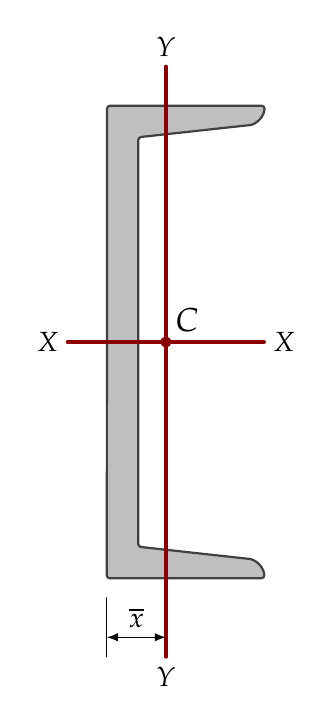
\begin{tikzpicture}[scale=\scale, line cap = round]
	\filldraw[rounded corners=1pt,draw=gray!50!black, fill=gray!50!white, thick] (0,0) -- (2, 0) arc(0:85:0.25) -- (0.4,0.4) -- +(0, 5.2) -- (1.775,5.75)arc(-85:0:0.25) -- +(-2,0) -- cycle;

	\draw[very thick, statsMaroon] (0.75,-1) -- (0.75,6.5);
	\draw[very thick, statsMaroon] (-0.5,3) -- (2,3);
	\fill[statsMaroon] (.75,3) circle (2pt) node[above right, black] {\large $C$};
	\node at  (-0.75,3) {$X$};
	\node at  (2.25,3) {$X$};
	\node at  (0.75,-1.25) {$Y$};
	\node at  (0.75,6.75) {$Y$};

	\draw (0,-.25) -- (0, -1);
	\draw[latex-latex] (0,-0.75) -- node[above] {$\overline{x}$} (0.75,-0.75);

\end{tikzpicture}

	}
	\hfill
	\mini[0.65]{
		\begin{itemize}

			\item The channel section has a horizontal axis of symmetry ($X-X$) but no vertical axis of symmetry.
			\item The centroidal $y$-axis is specified by $\overline{x}$ \lb(See the table A.5 in the course text for a particular section, sizes and corresponding properties.)
		\end{itemize}
	}

\end{frame}

%%%%%%%%%%%%%%%%%%%%%%%%%%%%%%%%%%%%%%%%%%%%%%%%%%%%%%%%%%%%%%%%%%%%%%%%%%%%%

\begin{frame}{Built-up Structural Steel Sections}
	\begin{myexam}{}{}
		\mini[0.5]{
			% !TEX root = ../all/statikz.tex

\tikz[scale=\scale]{
  \def\phil{gray!50!white}
  \def\stroke{black}

  \coordinate (A) at (-1.36,0);
  \coordinate (B) at (1.36,0);
  \coordinate (C) at (0,1.5);

  \Channel[180]{A}{\phil}{\stroke}{0.5}{1}
  \Channel{B}{\phil}{\stroke}{0.5}{1}
  \Channel[-90]{C}{\phil}{\stroke}{0.45}{1}
}

		}
		\hfill
		\mini[0.45]{
			Two C180X22 and one C150X19 are welded together as shown. \parb
			How far below the top of the built-up section is the centroidal $x$-axis?
			\parb
			\footnotesize
			\centering
			\textcolor{statsMaroon}{
			From the beam tables for C180X22:\lb
			Area $= 2790\,\mathsf{mm^2}$\lb
			Depth $=178\,\mathsf{mm}$\lb
			$\overline{x} =58\,\mathsf{mm}$\pars 
			From the beam tables for C150X19:\lb
			Area $= 2470\,\mathsf{mm^2}$\lb
			Depth $=152\,\mathsf{mm}$\lb
			$\overline{x} =54\,\mathsf{mm}$}
		}
		\addtocounter{\tcbcounter}{-1}
	\end{myexam}

\end{frame}

%%%%%%%%%%%%%%%%%%%%%%%%%%%%%%%%%%%%%%%%%%%%%%%%%%%%%%%%%%%%%%%%%%%%%%%%%%%%%

\begin{frame}{Built-up Structural Steel Sections}
	\begin{myexam}{Solution}{}
		\mini[0.35]{
		\def\scale{0.75}
			% !TEX root = ../all/statikz.tex

\tikz[scale=\scale]{
  \def\phil{gray!50!white}
  \def\stroke{black}

  \coordinate (A) at (-1.36,0);
  \coordinate (B) at (1.36,0);
  \coordinate (C) at (0,1.5);

  \draw[-latex] ($ (C)+(-2.5,0) $) -- +(5.5,0) node[above] {$x$};
  \draw[-latex] ($ (C)+(-0,-3.5) $) -- +(0,4.5) node[right] {$y$};

  \node at (-2,-0.5) {\footnotesize$A_1$};
  \node at (2,-0.5) {\footnotesize$A_2$};
  \node at (1,1.75) {\footnotesize$A_3$};

  \Channel[180]{A}{\phil}{\stroke}{0.5}{0.75}
  \Channel{B}{\phil}{\stroke}{0.5}{0.75}
  \Channel[-90]{C}{\phil}{\stroke}{0.45}{0.75}
}

		}
		\hfill
		\mini[0.55]{
			\centering\small
			\begin{tabular}{cccc}
				Shape    & $A_i$                            & $y_i$                          & $A_iy_i$                         \\
				         & \footnotesize$\mathsf{\;(mm^2)}$ & \footnotesize$\mathsf{\;(mm)}$ & \footnotesize$\mathsf{\;(mm^3)}$ \\
				\addlinespace
				\midrule
				$A_1$    & $2610$                           & $-101.5$                       & $-264920$                        \\
				\addlinespace
				$A_2$    & $2610$                           & $-101.5$                       & $-264920$                        \\
				\addlinespace
				$A_3$    & $1994$                           & $-12.67$                       & $-25264$                         \\
				\addlinespace
				\bottomrule
				\addlinespace
				$\Sigma$ & $7214$                           &                                & -$555104$
			\end{tabular}
			\parb
			\[ \overline{y} = \frac{\Sigma A_iy_i}{\Sigma A_i} = -76.948\text{ mm}\]
			\parb
			The centroidal $x$ axis is $76.9$ mm below the top of the plate.
		}

	\end{myexam}

\end{frame}

%%%%%%%%%%%%%%%%%%%%%%%%%%%%%%%%%%%%%%%%%%%%%%%%%%%%%%%%%%%%%%%%%%%%%%%%%%%%%

\begin{frame}{Built-up Structural Steel Sections}
	\begin{myexer}{}{}
		\mini[0.45]{
			\parm
			\def\scale{0.6}
			% !TEX root = ../all/statikz.tex

\tikz{
  
  \def\fill{gray!50!white}
  \def\draw{gray!50!black}
  \begin{scope}[scale=\scale]
    \begin{scope}
      \filldraw[rounded corners=1pt,draw=gray!50!black, fill=gray!50!white, thick] (0,0) -- (2, 0) arc(0:85:0.25) -- (0.4,0.4) -- +(0, 5.2) -- (1.775,5.75)arc(-85:0:0.25) -- +(-2,0) -- cycle;
    \end{scope}

    \begin{scope}[yshift=6cm, xshift=6cm]
      \filldraw[rounded corners=1pt,draw=gray!50!black, rotate=180, fill=gray!50!white, thick] (0,0) -- (2, 0) arc(0:85:0.25) -- (0.4,0.4) -- +(0, 5.2) -- (1.775,5.75)arc(-85:0:0.25) -- +(-2,0) -- cycle;
    \end{scope}

    \begin{scope}[yshift=6cm, xshift=6cm]
      \filldraw[rounded corners=1pt,draw=gray!50!black, fill=gray!50!white, thick, rotate=90] (0,0) -- (2, 0) arc(0:85:0.25) -- (0.4,0.4) -- +(0, 5.2) -- (1.775,5.75)arc(-85:0:0.25) -- +(-2,0) -- cycle;
    \end{scope}

    \filldraw[rounded corners=1pt,draw=gray!50!black, fill=gray!50!white, thick] (-.5,0) rectangle (0,8);

  \end{scope}
}

		}
		\hfill
		\mini[0.55]{
			Three C130 X 13 and a steel plate (12~mm~X~127~mm) are welded together. \parb
			Determine the location of the centroid, relative to the bottom left hand corner of the composite area.
			\parb
			\footnotesize
			\centering
			\textcolor{statsMaroon}{
			From the beam tables for C130X13:\lb
			Area $= 1700\,\mathsf{mm^2}$\lb
			Depth $=127\,\mathsf{mm}$\lb
			$\overline{x} =47\,\mathsf{mm}$}
		
		}
		\pars
	\end{myexer}

\end{frame}

% %%%%%%%%%%%%%%%%%%%%%%%%%%%%%%%%%%%%%%%%%%%%%%%%%%%%%%%%%%%%%%%%%%%%%%%%%%%%%%%%
% %%%%%%%%%%%%%%%%%%%%%%%%%%%%%%%%%%%%%%%%%%%%%%%%%%%%%%%%%%%%%%%%%%%%%%%%%%%%%%%%
% %%%%%%%%%%%%%%%%%%%%%%%%%%%%%%%%%%%%%%%%%%%%%%%%%%%%%%%%%%%%%%%%%%%%%%%%%%%%%%%%
% %%%%%%%%%%%%%%%%%%%%%%%%%%%%%%%%%%%%%%%%%%%%%%%%%%%%%%%%%%%%%%%%%%%%%%%%%%%%%%%%
% %%%%%%%%%%%%%%%%%%%%%%%%%%%%%%%%%%%%%%%%%%%%%%%%%%%%%%%%%%%%%%%%%%%%%%%%%%%%%%%%

\end{document}

%%%%%%%%%%%%%%%%%%%%%%%%%%%%%%%%%%%%%%%%%%%%%%%%%%%%%%%%%%%%%%%%%%%%%%%%%%%%%%%%